\documentclass[conference]{IEEEtran}
\IEEEoverridecommandlockouts
% The preceding line is only needed to identify funding in the first footnote. If that is unneeded, please comment it out.

%\usepackage{cite}
\usepackage[numbers,sort&compress]{natbib}
\usepackage{amsmath,amssymb,amsfonts}
\usepackage{algorithmic}
\usepackage{graphicx}
\usepackage{textcomp}
\usepackage{epsfig,endnotes}
\usepackage{tikz}
\usepackage{multirow}
\usepackage{booktabs}
\usepackage{dirtytalk}
\usepackage{rotating}
\usepackage{verbatim}
\usepackage{xspace}
%\usepackage[title]{appendix}
\usepackage{enumitem}
\usepackage{xcolor}
\usepackage{colortbl}
\usepackage{url}
%\usepackage[page]{appendix}

\urlstyle{rm}  

\def\UrlBreaks{\do\A\do\B\do\C\do\D\do\E\do\F\do\G\do\H\do\I\do\J
\do\K\do\L\do\M\do\N\do\O\do\P\do\Q\do\R\do\S\do\T\do\U\do\V
\do\W\do\X\do\Y\do\Z\do\[\do\\\do\]\do\^\do\_\do\`\do\a\do\b
\do\c\do\d\do\e\do\f\do\g\do\h\do\i\do\j\do\k\do\l\do\m\do\n
\do\o\do\p\do\q\do\r\do\s\do\t\do\u\do\v\do\w\do\x\do\y\do\z
\do\.\do\@\do\\\do\/\do\!\do\_\do\|\do\;\do\>\do\]\do\)\do\,
\do\?\do\'\do+\do\=\do\#}

\DeclareMathOperator*{\argmax}{arg\,max}
\DeclareMathOperator*{\argmin}{arg\,min}

\def\BibTeX{{\rm B\kern-.05em{\sc i\kern-.025em b}\kern-.08em
    T\kern-.1667em\lower.7ex\hbox{E}\kern-.125emX}}
\newcommand{\commentout}[1]{}    
\newcommand{\us}{\textbf{SimEngine}\xspace}     
% macros for nice i.e., e.g., and et al.
\newcommand{\ie}                {\emph{i.e.},\xspace}
\newcommand{\eg}                {\emph{e.g.},\xspace}
\newcommand{\etal}              {\emph{et~al.}\xspace}
\newcommand{\naive}             {na\"{\i}ve\xspace}
\newcommand{\Naive}             {Na\"{\i}ve\xspace}
%%%%%%%%%%%%%%%%%%%%%%%%%%%%%%%%%%%%%%%%%%%%%%%%%%%%%%%%%%%%%%%%%%%%%%%%%%%%%%
% Define extra colors
\definecolor{darkgreen}{rgb}{0,0.5,0}
\definecolor{purple}{rgb}{0.75,0,0.75}
\definecolor{brown}{rgb}{0.65,0.16,0.16}
\definecolor{darkslateblue}{rgb}{0.28, 0.24, 0.55}
\definecolor{orange}{rgb}{1.0, 0.647, 0}

% Add Cite or Ref placeholder macros
% conflicts with other latex packages.
\newcommand{\ac}[1]       {\fslnote{CITE}{magenta}{#1}}
\newcommand{\addref}[1]        {\fslnote{REF}{magenta}{#1}}

\newcommand{\avani}[1]          {\textcolor{darkslateblue}{[Avani:#1]}}
\newcommand{\jeanine}[1]           {\textcolor{purple}{[Jeanine:#1]}}
\newcommand{\omar}[1]           {\textcolor{orange}{[Omar:#1]}}
\newcommand{\si}[1]           {\textcolor{darkgreen}{[Si:#1]}}
\newcommand{\steen}[1]           {\textcolor{gray}{\textbf{[Steen:#1]}}}


\newcommand{\todo}[1]           {\textcolor{red}{[TODO:#1]}}

\begin{document}

\title{\Large \bf Beyond Guess and Check: Quantifying Fidelity of Proxy Applications\\

% \thanks{Identify applicable funding agency here. If none, delete this.}
}

\commentout{ %---anonymous submission-----
\author{\IEEEauthorblockN{1\textsuperscript{st} Si Chen}
\IEEEauthorblockA{
\textit{Emory University}\\
Atlanta, GA, USA \\
si.chen2@emory.edu}
\and
\IEEEauthorblockN{2\textsuperscript{nd} Omar Aaziz}
\IEEEauthorblockA{
\textit{Sandia National Laboratories}\\
Albuquerque,New Mexico,USA\\
oaaziz@sandia.gov}
\and
\IEEEauthorblockN{3\textsuperscript{rd} Jeanine Cook}
\IEEEauthorblockA{
\textit{Sandia National Laboratories}\\
Albuquerque,New Mexico,USA\\
jeacook@sandia.gov}
\and
\IEEEauthorblockN{4\textsuperscript{th} Avani Wildani}
\IEEEauthorblockA{
\textit{Emory University}\\
Atlanta, GA, USA\\
avani@mathcs.emory.edu}

}
}%------end comment out-------
\maketitle

\begin{abstract}
%Proxy applications are smaller models of a larger parent application that are targeted to represent particular characteristics such as programming model or node, memory, or communication behavior of the parent. They are widely used in HPC hardware/software co-design as code development tools, and in system acquisition as performance benchmarks. We often accept, qualitatively, that proxies are faithful representations of their parents, but this has little quantitative validation. In this work, we propose a framework called \us to quantitatively demonstrate the correspondence of proxy to parent in their underlying node and memory hardware behavior. \us implements similarity algorithms to compare application behavior, and Laplacian score with correlation filter to select the most important features. It is a robust framework to characterize behavioral similarities that can be applied to many problems in the HPC context.Using the selected concise features, we show that 75\% of the proxies in our suite demonstrate highly convergent behavior with respect to their parents, and therefore, are faithful representations.
%\us is a robust framework to determine behavioral similarities that can be applied to many problems in the HPC context.  
Proxy applications are smaller models of a larger parent application, targeted to represent characteristics such as the programming model, or node, memory, or communication behavior of the parent. They are widely used in HPC hardware/software co-design as code development tools, and in system acquisition as performance benchmarks. We often accept, qualitatively, that proxies are faithful representations of their parents, but this has little quantitative validation. In this work, we propose \us, a robust framework to characterize behavioral similarities that can be applied to many problems in the HPC context. \us implements similarity algorithms to compare application behavior, and Laplacian score with a correlation filter to select the most important application features. Using the selected concise features, we show that 75\% of the proxies in our suite demonstrate highly convergent behavior with respect to their parents, and therefore, are faithful representations.
\end{abstract}

\begin{IEEEkeywords}
Co-design, Performance analysis, proxy/parent representativeness

\end{IEEEkeywords}

\section{Introduction}
\label{sec:intro}
HPC applications tend towards being both large and complex, with numerous dependencies and significant footprints on infrastructure.
Using these applications to drive activities such as HPC system co-design, procurement and acceptance testing~\cite{larrea2020towards}, explorations of communication bottlenecks~\cite{aaziz2019fine}, or varying programming models~\cite{hochstein2005parallel}, can be daunting and very time-consuming in the face of such complexity.

An obvious approach to this problem is to design \emph{proxy applications}, applications designed to represent some (and, crucially, not all) behaviors or characteristics of a parent application, but with fewer lines of code and dependencies.  Proxy applications have additional benefits for access control; they can often be made open source while representing characteristics of export-controlled code, opening more avenues for measurement and analysis of controlled HPC environments outside secured settings.
%%
%
%with are smaller (fewer lines of code), less complex (fewer dependencies) applications that are specifically designed to represent some behavior or characteristic of a larger, more complex parent application.  
%They were originally developed so that researchers throughout the HPC community could have a smaller, more tractable code to work with  that has no access controls (i.e.,
%they are open-source and can represent characteristics of export-controlled code).
%Some proxies are designed solely to investigate a particular programming model(s), while for other proxies, the communication behavior may be the important bottleneck in the parent application, so this behavior is accurately implemented in the proxy. 
%It is important to note that many proxies are not intended to represent every aspect of their respective parents.

%Proxy applications have also become widely used for many activities
%including system co-design and procurement.   The 
%national laboratories directly engage in co-design with many of the 
%primary computer system vendors. 
% OMAR: This paragraph is to the point but as someone don't understand procurement means and don't have time to look into the words. It may skipped by the reviewers.

%Proxy applications have also become widely used for many activities including HPC system advance design, procurement and acceptance testing. 
The national laboratories directly engage in co-design with many of the primary computer system vendors. The goal of these efforts is to optimize the performance of target applications on the vendor system designs in development.\avani{I think we can cut this paragraph before here, and possibly entirely, but I'd like opinions.} \jeanine{I think this provides some primary motivation and I would not cut.}
%
A suite of proxy apps is often the contracted benchmark suite used to optimize system performance, with the assumption that this will in turn optimize target application performance on the system.
%For this, we need to ensure that the proxy applications used are high fidelity models of the target parent applications, since vendors are developing designs to optimize performance primarily based on proxies.  
%
If the communication, memory, and/or node behavior of the parent applications are very different than that of the proxies, the result could be a system that has highly sub-optimal parent application performance. This also applies to procurement activities, where the system procured is often that which optimizes the performance of the proxy application suite given to potential vendors.  
 

Proxy applications are freely available from many different organizations, many of which are catalogued in the ExaScale Computing Project (ECP)~\cite{ECPProxySuite1}.  There is strong motivation to minimize the number of proxy applications that maximize the range of application behaviors of interest, since more proxies mean more time and effort in both co-design and procurement. However, narrowing down the suite of proxies used in these processes can be difficult, and is often based on purely qualitative expertise, with no real quantitative data to support these decisions. 

%Thus the two main research questions being addressed here are how closely proxy behavior on a system represents parent behavior, and how similar proxies are to each other so that a co-design or procurement suite does not suffer from redundancy. Moreover, gaps can be identified when there is no proxy that represents the behavior of an application.
%or gaps.
The three main research questions we address are: how closely proxy behavior on a system represents parent behavior, how similar proxies are to each other so that a co-design or procurement suite does not suffer from redundancy, and how to identify gaps, where there is no proxy that represents the behavior of a parent application.

We introduce \us to determine the similarity between proxy and parent applications. We generalize the engine for more comprehensive usage in the HPC area, as well as implement several similarity algorithms and demonstrate how to choose the best algorithm for a given dataset \jeanine{Then we need tp demonstrate this.  Right now we say that all of the algorithms return pretty much same results so we choose the simplest.  What about a ground truth discussion somewhere?} We also include algorithms to facilitate feature selection, as minimizing the number of features is very important to reduce the data collected and thus lower the number of application runs.
%We pose that cosine similarity is the preferred algorithm for our data because of its simplicity, performance, and ease of interpretability by geometric angle. Without knowing which hardware events are more representative, we exhaustively collect all the events that the platforms can provide. 
%In order to simplify the data collection process and enable cross-platform comparison, we aim to find a concise event subset.\us combines Laplacian score~\cite{he2005laplacian} to rank the important features and the Pearson correlation to remove the correlated features.
With the help of quantitative similarity measurement in \us, users are guided to choose proper proxy applications for particular uses. Besides quantifying fidelity of proxy applications, similarity measurement approaches in \us can also be applied to various HPC problems, such as compiler optimization, code refactoring, and application input sensitivity.


Our primary contributions include:
\begin{enumerate}
    \item The first comprehensive characterization of proxy application fidelity at a hardware level using ML-based similarity algorithms and a large suite of ECP proxy/parent application pairs. %to present a comparison of similarity measurements(\S~\ref{sec:SimCom}) to quantitatively demonstrate proxy fidelity.
    \item 
    %The features in our FIXME traces and reduce dimensionality by 95\%. 
    Identification of important features that reduce the dimensionality of the data set by 95\%.
    \item The \us toolkit and data collection infrastructure are publicly available for similarity measurements and collection, and are actively used and deployed on HPC production systems. %\todo{Need strength}
\end{enumerate}


\section{\us}
\label{sec:simEngine}
%Our fundamental question in this work is 
To determine how similar proxy and parent applications behave in terms of resource utilization such as computation and memory, we explore the use of several ML similarity techniques. Those techniques work differently, making it hard to determine which one reveals the real relationship, so we create \us to intercept the level of agreement between those techniques that could reflect the accurate answer. 
%\todo{why we need to use several similarity techniques?}
%A fundamental question we pose is: ``how similar are applications to each other in the way they utilize system resources, particularly computation and memory?''
%, with a focus in this work on node computation and memory resources. 
%We introduce a framework \us to determine this similarity between proxy and parent applications.
%Figure~\ref{figs:us} shows the workflow of \us.

We collect hardware performance counters from several proxy, parent applications, and benchmarks to provide a comprehensive collection of informational measurements that reveals the application execution resources fingerprints to determine similarity.  
Figure~\ref{figs:us} shows the workflow of \us, where we use Lightweight Distributed Metric Service (LDMS)~\cite{ldms_sandia} as the data collection framework to collect PAPI HW performance counters from HPC applications. Then, LDMS send the data to the feature selection layer as a data matrix $X$ that has $n$ rows of application vectors $x_{1},\ldots,x_{n}$ and features $f_{1},\ldots,f_{d}$ as the columns.

%a vector $x_{i}$ with the length of $d$ dimensions ($d$ being the number of hardware events), and build a data matrix $X$ that has $n$ rows of application vectors $x_{1},\ldots,x_{n}$. The columns of $X$ are the features $f_{1},\ldots,f_{d}$.

During feature selection, we rank the features by calculating importance scores and select the important $k$ features by a correlation filter.
The matrix $X'$, which has k features as the columns, preserves the similarity structure of the matrix $X$. 
Finally, using the selected important features, we produce similarity matrices to compare the similarity between applications and quantify the fidelity of proxy and parent applications. 
%Our analysis tools that compute feature ranking, correlation filter, and similarity measurement are written in python and use several of the standard math libraries (\eg math, numpy) and scikit-learn facilities.  We have also developed an extensive infrastructure to automate data collection experiments.\todo{possibly move this paragraph to artifact evaluation}

\begin{figure}[ht]
\centering
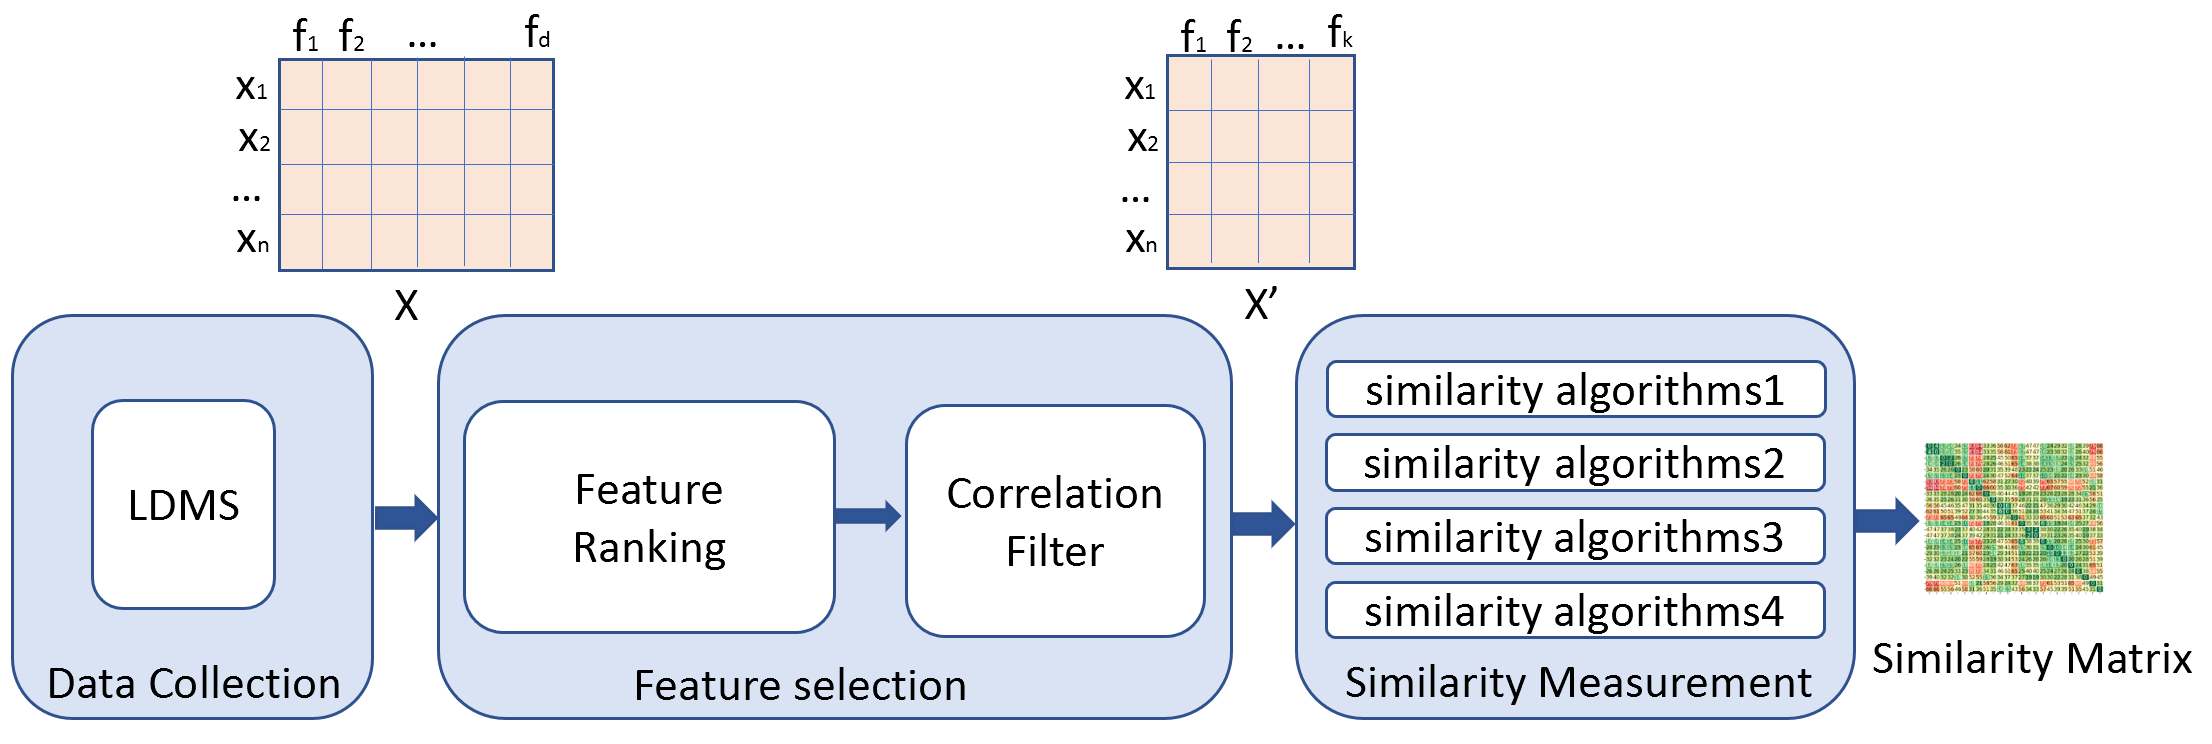
\includegraphics[width=\linewidth]{figs/SimEngine.png}
\caption{\us Architecture }
\label{figs:us}
\end{figure}

\subsection{Similarity and Distance}
\label{sec:Sim}

Evaluating the similarity between proxy and parents is one of the main goals of our work.
For each application, we sample, by second, the accumulated hardware counters, for the whole execution. Then we average the last 5 seconds of the application execution for each event across ranks. Thus, we get an application vector $x_{i}$, that contains a series of averaged hardware event counters (\ie $x_{ik}$). 
%\todo{sentence about how we represent applciations as vectors} .
We define two applications as \emph{similar} if the vectors that represent the applications are a short distance apart, which, in many classification tasks, corresponds to the vectors belonging to the same class. %The similarity is defined using a distance measure. 
After calculating the pairwise distance between each application pair, we get a similarity matrix. %We expect the diagonal of the matrix to be zero, as that the distance of the vectors between the applications and themselves. 
Finally, we compare the result of four typical similarity metrics, introduced below, and choose the metric that most accurately correlates known proxy/parent pairs. 

\commentout{
\subsubsection{Background}
\todo{this is mostly untested metrics, right?  Why is it here?}
We define two vectors as \emph{similar} if they are a short distance apart, which, in many classification tasks, corresponds to the vectors belonging to the same class.
%of two vectors in space is called similarity. If two vectors are similar, their distance is short, and vice versa.
%In many classification tasks, the samples with short distances are intuitively similar to each other and more likely belong to the same class.
%
%
The most familiar distance metrics are Minkowski distances, where the distance $D$ between two vectors $X$ and $Y$ is defined as $(\sum_{i=1}^n|x_i-y_i|^p)^{1/p}$, which reduces to Manhattan distance at $p=1$ and Euclidean distance at $p=2$~\cite{9distance}. 
%In some scenarios, normalization is needed to overcome the magnitude variant on each feature. 
In high dimensional space, Minkowski distances for small $p$ become less useful because of the curse of dimensionality -- all of the points are about the same distance. Cosine similarity (\S\ref{sec:cos_sim}) has often been used as a way to counteract these drawbacks since the magnitude of vectors is not taken into account. After Z-score standardization, we could consider Pearson correlation, Cosine similarity, and Euclidean distance as equivalent.\avani{previous is unclear} %Minkowski distance is a group of distance metrics, which with some parameters it turns into Manhattan distance, Euclidean distance, and Chebyshev distance. %Undoubtedly, choosing the best parameter is not trivial and depends on use cases. 
The Jaccard Index calculates the similarity and diversity of two sample sets, which are heavily impacted by the size of data. Hamming distance is typically used to compare two binary strings.\avani{why are you telling me about Hamming distance?}

\avani{cut text below for space (see comments in tex)}
%Another big category of distance is statistical distance~\cite{statdis}. Mahalanobis distance~\cite{Mah} is an effective multivariate distance metric that measures the distance between a point (vector) and a distribution or two points from the same distribution. 
%
%It could eliminate the correlation between features. Kullack-leibler divergence~\cite{kullback1951information}, Jensen-Shannon divergence~\cite{endres2003new}, and Wasserstein distance\cite{rubner2000earth} are widely used to minimize the loss function when updating Machine Learning models. 
%
%Obviously, if we use different distance measurements, we would get different distances. Depending on the way we represent the objects of a clustering, we need to find the most appropriate distance metric to achieve the best result for our specific task.
}%------end comment out-------

\subsubsection{Cosine Similarity}
\label{sec:cos_sim}
Cosine similarity compares the angle between vectors in an inner product space, where the inner product can be conceptualized
as the projection of one vector $x_{i}$ in the direction of the other vector $x_{j}$. The calculation relies on the two complementary definitions (algebraic and geometric) for computing the inner product:
\begin{itemize}
\item 
Algebraic Inner Product:
$x_{i}\cdot x_{j}=\sum_{k=1}^{d} x_{ik} x_{jk}$
\item
Geometric Inner Product:
$x_{i}\cdot x_{j}=\|x_{i}\|\|y_{i}\|\cos\theta$
\item
Cosine Similarity:
\begin{equation}
\cos(\theta)=\frac{\sum_{k=1}^{d} x_{ik} x_{jk}}{\|x_{i}\|\|x_{j}\|}
\end{equation}
\end{itemize} 
%Cosine similarity compares the angle between two vectors $x_{i}$ and $x_{j}$ using vector inner product. 
The cosine varies from 1.0 (identical vector direction) to 0.0 (orthogonal vectors), and the degree $\theta$ varies from 0 (similar) to 90 (dissimilar). If two applications have similar behavior then we are expecting their cosine similarity angle to be closer to 0 degree.  

\subsubsection{Jensen-Shannon (JS) Divergence}
\label{sec:JS}
Instead of comparing two vectors, we can normalize each vector and think of it as a probability distribution (each event turns into a probability), and then compare the two distributions.
JS divergence~\cite{endres2003new} measures the distance between two probability distributions $P$ and $Q$. JS divergence is a generalization of  Kullback–Leibler (KL) divergence~\cite{kullback1951information}, the relative entropy from distributions $Q$ to $P$, \ie the expectation of the logarithmic difference between the probability distributions $Q$ and $P$. 
\begin{align*}
KL(P|Q)&=\sum_{x} P(x) \log \frac{P(x)}{Q(x)} \\ 
&=-\sum_{x} P(x) \log {Q(x)}+\sum_{x} P(x) \log {P(x)} \\ 
& =\textrm{cross entropy – entropy}
\end{align*}
KL divergence is asymmetric and has no upper bound. Unlike KL divergence, JS divergence is symmetric and returns a value between 0 and 1, where 0 means similar and 1 is diverge. %both of which are valuable properties for application comparison. 
JS divergence is defined as 
\begin{equation}
\operatorname{JS}(P \| Q)=\frac{1}{2} KL(P \| M)+\frac{1}{2} KL(Q \| M)
\end{equation}
where $M=\frac{1}{2}(P+Q)$.% JS divergence calculates total KL divergences in two directions to the average.  

\subsubsection{Wasserstein Distance}
\label{sec:wass}
Wasserstein distance\cite{rubner2000earth} can be interpreted as the minimum ``cost'' of transforming a probability distribution $P$ into distribution $Q$, where ``cost'' is measured as the amount of distribution weight that must be moved, times the distance it has to be moved~\cite{wassersteinscipy}. 
Unlike other statistic distances like JS divergence, Wasserstein distance multiplies the probability distribution and the distance, thus the order of the events matters. 
%If the events that have divergent behaviour located far away in the vectors, the Wasserstein distance is bigger. 
Since Wasserstein distance does not require both measures to be in the same probability space (\ie, two vectors may have different lengths), it can be used to compare application performances across platforms that support a different number of hardware event counts. The $p^{th}$ Wasserstein distance is defined as 
\begin{equation}
W_{p}(P, Q)=\left(\inf _{J \in \mathcal{J}(P, Q)} \int\|x-y\|^{p} d J(x, y)\right)^{1 / p}
\end{equation},
where $\mathcal{J}(P, Q)$ denotes all joint distributions $J$ for $(X,Y)$ that have marginals $P$ and $Q$. Generally, when $p = 1$ and $d = 1$, we compute the first Wasserstein distance between two 1-dimensional distributions, which is also known as earth mover distance. Wasserstein distance does not have upper bound, where 0 means similar and bigger value means dissimilar.

\subsubsection{Mahalanobis Distance}
Mahalanobis distance~\cite{Mah} is an effective multivariate distance metric that measures the distance between a point (vector) and a distribution, or two points from the same distribution. 
The Mahalanobis distance~\cite{Mah} between two vectors $x_i$ and $x_j$ from the same distribution is defined as
\begin{equation}d_{M}(x_i, x_j)=\sqrt{(x_i-x_j)^{T} S^{-1}(x_i-x_j)}
\end{equation}, where $S$ is the covariance matrix of the data set. Geometrically, it transforms the data by whitening and normalizing the covariance and computes the ordinary Euclidean distance for the transformed data. Since the Mahalanobis distance accounts for the variance of each variable and the covariance between variables, it is used in areas such as multivariate anomaly detection and imbalanced classification. Note that the Mahalanobis distance requires more samples than features to calculate the covariance matrix. Thus, we reduce features with principal components analysis (PCA) before applying Mahalanobis distance. Mahalanobis distance also does not have upper bound, where 0 means similar and bigger value means dissimilar.

\subsection{Feature Selection}
The data collection process is torture in our experiment. Without knowing which hardware events are more representative, we exhaustively collected all the events that the platforms could provide, which is around 500 hardware events for each application on platform Intel Skylake. 
By Occam’s Razor, the simplest model that explains a situation is the correct approach. 
Irrelevant features may increase noise and reduce the accuracy of a model, while adding to latency, storage overhead, and the amount of data processing. There are two classes of algorithms to reduce a feature space: feature extraction and feature selection. 
Feature extraction, which recombines original features into a denser set, retains the overhead of data collection and sacrifices interpretability, so we focus on feature selection. Feature selection speeds up algorithms, improves accuracy, and enhances comprehensibility~\cite{guyon2003introduction}. 

%Feature extraction is to find a smaller set of new variables, each being a combination of the original features. Because feature extraction still requires collecting all the features and loses interpretability, it is not what we are looking for. 

%\avani{I propose we cut the rest of this paragraph}
%Feature Selection can be categorized into filter methods, wrapper methods, and embedded methods. The filter methods always focus on the intrinsic properties (\eg Variance) of data itself, which are more suitable for unsupervised learning. %Examples of filter methods include Information Gain, Chi-square Test, Fisher’s Score, Correlation Coefficient, Variance Threshold, Mean Absolute Difference, and Dispersion ratio. 
%Wrapper methods evaluate features by applying a selection algorithm and comparing the final value with the target value. They require a greedy search in the feature space. The typical wrapper method is Recursive Feature Elimination\cite{guyon2002gene}. Embedded methods, such as Random Forest\cite{ho1995random}, get the important features while interactively building up the model. Most of the wrapper and embedded feature selection methods are designed for supervised learning. 
To simplify the data collection process and enable cross-platform comparison, we aim to find a concise event subset. \us uses Laplacian score~\cite{he2005laplacian} to rank the important features, combined with the Pearson correlation to remove the correlated features.

\subsubsection{Feature Score}
\label{sec:feature_score}
Consider a data matrix $X$ that has $n$ rows of samples with $d$ dimensions $x_{1},...,x_{n}$. The columns of $X$ are the features $f_{1},...f_{d}$. Our goal is to find the subset of $k$ important features which preserve the similarity structure of the matrix $X$. 

%Since we lack ground truth for the class label for each application, the filter method of feature selection is more suitable.
Since we are only interested in maintaining the similarity relationship between the proxy/parent application pair points, but not concerned about the dissimilarity of non-proxy/parent application pair points, neighbor embedding is the perfect unsupervised method for this task. We choose a graph-based feature ranking technology called Laplacian score~\cite{he2005laplacian} to compute the importance of features.  Laplacian score builds a nearest neighbor graph for application points and seeks those features that respect local graph structure. In our case, these features help preserve the neighbor similarity between proxy and parent applications.  

The Laplacian score of the $r^\textrm{th}$ feature can be expressed as:
\begin{equation}L_{r}=\frac{\widetilde{\mathbf{f}}_{r}^{T} L \widetilde{\mathbf{f}}_{r}}{\widetilde{\mathbf{f}}_{r}^{T} \widetilde{\mathbf{f}_{r}}}
\end{equation}
, or in a more understandable way:
\begin{equation}
L_{r}=\frac{\Sigma_{i j}\left(f_{r i}-f_{r j}\right)^{2} S_{i j}}{\operatorname{Var}\left(\mathbf{f}_{r}\right)}
\end{equation} , where $f_r$ is the $r^\textrm{th}$ feature, and $S_{i j}$ is the weight matrix. An element $S_{i j}$ will only have a nonzero value $S_{i j}=e^{-\frac{\left\|\mathrm{x}_{i}-\mathrm{x}_{j}\right\|^{2}}{2t^{2}}}$ when $i$ and $j$ are neighbors, otherwise the value of that entry is zero. $t$ is a user-defined bandwidth, with $1$ as a default value. The denominator indicates the variance of the $r^\textrm{th}$ feature; larger values correlate to more information represented. The numerator indicates the sum of feature value differences within the points' neighbors; here, the smaller the Laplacian score is, the more important the feature is. Finally, we get the ranked features sorted by Laplacian score.

Since features are evaluated separately in the Laplacian score, if we select features with the smallest Laplacian score, some redundant features may be included. To select an informative set of important features in order to optimize combination performance, we introduce the correlation filter.

\subsubsection{Correlation Filter}
When a group of features are highly correlated, we only need to include one in our selection. A broadly used correlation measure is the Pearson correlation coefficient (PCC). PCC measures the linear correlation between two variables $f_{i}, f_{j}$. 
\begin{equation}
\rho_{f_{i}, f_{j}}=\frac{\operatorname{cov}(f_{i}, f_{j})}{\sigma_{f_{i}} \sigma_{f_{j}}}
\end{equation}
where $\operatorname{cov}$ is the covariance and $\sigma_{f_{i}}$is the standard deviation of $f_{i}$.
PCC has a value between +1 and -1, where +1 is a total positive linear correlation, 0 is no linear correlation, and -1 is a total negative linear correlation. We choose a PCC threshold of 0.9 because we want to keep reasonable number of important features while removing strongly correlated ones.  

We calculate the pairwise PCC for all ranked features and fetch features one by one from the ranked feature to our important feature subset. Each time we select one feature, we remove the redundant features with PCC $> 0.9$ or $< -0.9$ from the remaining features. We stop collecting features when there are no more features in the feature pool. %we obtain a pre-selected number, or when there are no more features in the feature pool.

Note that the PCC can evaluate only a linear relationship between two continuous variables; we will investigate more correlation methods in future work.
\section{Experiment Platform}
\label{sec:expPlatform}
In this section, we present our methodology for collecting data and 
how we use that data to perform similarity analysis using \us.  We use
an Intel Skylake production HPC system to collect
data on 21 proxy and parent applications that span several scientific
domains.  We also collect data on several standard HPC benchmarks and 
use these in our analysis to provide a baseline for aiding in understanding the results.
 
\subsection{Application Suite}
Of the applications used in this work, some are proxy/parent pairs and
some are proxies or parents that are not paired. We also include several
standard HPC benchmarks.
Not all applications
we use are proxy/parent pairs because some proxies 
have export-controlled parents for which data cannot be 
publicly released.  Also, Castro is the parent of a 
proxy called Thornado~\cite{ECPProxySuite1}, but at this point, we are not
using Thornado because of I/O issues within the code that caused problems with 
data collection.
\cite{ECPProxySuite1}.

We use the Intel compiler to build
all of the applications except OpenMC.  
On the Intel Skylake system, we use \emph{icc} 20.0.2.254 and
\emph{OpenMPI} 4.0.3.  OpenMC requires the use of 
the 8.3.1 GNU compiler, due to inherent constraints
within the code.

For each proxy/parent pair,
we use the same input problem and/or parameters where possible. 
In cases where we cannot run the same problem, we use the closest 
matching problem available and we size both proxy and parent application
problems in all cases to use about 50\% of the available memory.   

\definecolor{Gray}{gray}{0.9}
\begin{table}[!t]
\scriptsize
\caption{Proxy/Parent version information}
\label{tab:versions}
\centering
\begin{tabular}{ll|ll}
\toprule
\textbf{Proxy}                                  & \textbf{Version}                          & \textbf{Parent}                       & \textbf{Version}                           \\ 
\midrule
AMG2013~\cite{AMG}                    & \cellcolor{Gray!50}2013\_0       & N/A                                         & \cellcolor{Gray!50}N/A                 \\
N/A                                                 & \cellcolor{Gray!50}N/A               & Castro~\cite{Castro}               & \cellcolor{Gray!50}20.07              \\
ExaMiniMD~\cite{ostiExaMiniMD}        & \cellcolor{Gray!50}1.0               & LAMMPS~\cite{LAMMPS}      & \cellcolor{Gray!50}17 Aug 2017   \\
Laghos~\cite{Laghos}                     & \cellcolor{Gray!50}3.0               & N/A                                          & \cellcolor{Gray!50}N/A                  \\
miniQMC~\cite{richards2018fy18}  & \cellcolor{Gray!50}0.4               & QMCPACK~\cite{qmcpack}    & \cellcolor{Gray!50}3.8                  \\
miniVite~\cite{miniVite}                    & \cellcolor{Gray!50}1.0               & Vite~\cite{Vite}                        & \cellcolor{Gray!50} 30 Sept 2020  \\
Nekbone~\cite{nekbone}                 & \cellcolor{Gray!50} 3.1               & Nek5000~\cite{Nek5000}        & \cellcolor{Gray!50}19.0                 \\
PENNANT~\cite{pennant}               & \cellcolor{Gray!50}0.9                & N/A                                          & \cellcolor{Gray!50} N/A                 \\
PICSARlite~\cite{picsarlite}             &\cellcolor{Gray!50}16 July 2020  & PICSAR~\cite{PICSAR}         & \cellcolor{Gray!50}16 July 2020    \\
SNAP~\cite{snap}                            & \cellcolor{Gray!50}1.09              & N/A                                          & \cellcolor{Gray!50}N/A                  \\
SW4lite~\cite{ECPProxySuite1}        & \cellcolor{Gray!50}2.0                & SW4~\cite{SW42}                  & \cellcolor{Gray!50}2.0                    \\
SWFFT~\cite{ECPProxySuite1}  & \cellcolor{Gray!50}1.0                & HACC~\cite{HACC}                & \cellcolor{Gray!50} 1.0                 \\
XSBench~\cite{XSBench}               & \cellcolor{Gray!50}19.0               & OpenMC~\cite{OpenMC}       & \cellcolor{Gray!50}0.11.0             \\
HPCG benchmark~\cite{hpcg}        &  \cellcolor{Gray!50}3.1                & N/A                                         &  \cellcolor{Gray!50}N/A                \\
HPCC benchmark~\cite{hpcc}        &  \cellcolor{Gray!50}1.5.0             & N/A                                          &  \cellcolor{Gray!50}N/A               \\
\bottomrule
\end{tabular}
\end{table}

Table~\ref{tab:versions} contains all of the proxy/parent pairs and other
applications and the specific versions that we use in this work. If a
date is given, it is the latest code available in the repository at
that date.

\jeanine{I put the descriptions of the applications in, but we can delete
if we need the space.}
AMG2013~\cite{AMG} is a proxy application for BoomerAMG and is a parallel
algebraic multigrid solver for linear systems arising from unstructured grid
problems.  %We are using version 2013\_0 and are running 
We ran the default Laplace problem with a custom resizing.
We did not run BoomerAMG because we did not have the expertise to 
ensure that we treated it fairly, but we intend to use it in the future.
%
LAMMPS~\cite{LAMMPS} is a classical molecular dynamics code, 
%that models particles in solid, liquid, and gas states.  A 
with particles ranging from a single atom to a large composition of material.  
%LAMMPS integrates Newton's equations of motion to model particle interaction, using lists to track neighboring particles. 
It implements mostly short-range solvers, but does include some methods for long-range particle interactions.  
ExaMiniMD~\cite{ostiExaMiniMD}, which is  
a proxy for LAMMPS, %uses spatial domain decomposition but 
implements limited types of interactions, and only short-range ones.
%ExaMiniMD and LAMMPS both use neighbor lists for the force calculation. ExaMiniMD is intended to represent both the computation (including memory behavior) and communication that is implemented in LAMMPS. 
%
Laghos~\cite{Laghos} is a proxy application that is a high-order Lagrangian
hydrocode meant to represent several compressible shock hydrocodes, including BLAST.
%We ran version 3.0 of the code using libraries: hypre
%version 2.11.2, metis version 4.0.3, and mfem version 4.1.1.  
%The problem that we are running is 
%We ran the Sedov blast wave problem with partial assembly. 
We did not
run BLAST because it is export controlled and we are still working with LLNL
to run its experiments on their systems.
%
QMCPACK~\cite{qmcpack} is a quantum Monte Carlo package for computing the electronic structure of atoms. MiniQMC~\cite{richards2018fy18} 
%is a simplified computational proxy covering 
covers QMCPACK's essential computational kernels. The computational themes of miniQMC and QMCPACK are particle methods, dense and sparse linear algebra, and Monte Carlo methods.
% Both implement Variational Monte Carlo, and diffusion Monte Carlo advanced QMC algorithms.
%
Vite~\cite{Vite} is an implementation of Louvain method for (undirected)
graph clustering or community detection.  
%The version we ar running was pulled from the repository on September 30, 2020.  
MiniVite~\cite{miniVite} is a proxy application for Vite that implements a
single phase of the Louvain method in distributed memory for community
detection. 
%We ran both over the same large random graph generated using other tools.
%We are running version 1.0 and running 
%We ran it with the same random graph as Vite.
%
Nek5000~\cite{Nek5000} is a spectral element computational fluid dynamics
solver while its proxy application Nekbone solves the Poisson equation with
a spectral element multigrid preconditioned conjugate gradient solver.  
%We are using version 19.0 of Nek5000 and are running 
%% we are using version 17.0 of Nekbone with 
%With Nek5000 we ran an eddy test problem and 
%for Nekbone ran an expanded version of the example2 test problem.
%
% NEED PENNANT and bibtex
PENNANT~\cite{pennant} serves as a proxy application for rad-hydro physics-based algorithms on an unstructured mesh, modeling the computation and memory access patterns typical to rad-hydro applications. It is modeled on, and thus serves as a proxy for, the LANL code FLAG.
%
PICSAR~\cite{PICSAR} is Particle-In-Cell solver, while its proxy
application, PICSARlite~\cite{picsarlite}, is a subset of the actual codebase.  
%We are using a version of the code that was pulled from the repository on July 16, 2020.
%We ran a resized version of the homogeneous\_plasma\_lite problem for both of
%the codes.
%
% NEED SNAP and bibtex
SNAP~\cite{snap} serves as a proxy application for discrete ordinates neutral particle transport, modeling the computation and memory access patterns typical to neutral particle transport applications. It is modeled on, and thus is a proxy for, the LANL code PARTISN.
%
SW4~\cite{SW42} is a geodynamics code that solves 3D seismc wave equations with local mesh refinement.
%enables 3D modeling of surface topologies to understand the physics and impacts of earthquakes and other seismological events.  The seismic wave equations are solved on locations that are specified either by Cartesian or geographic coordinates.
%The finite difference wave equations numerically simulate wave propagation to fourth-order, which is very accurate for calculating surface waves.  Cartesian local mesh refinement is used to improve accuracy in regions near the free surface, where more resolution is needed to solve short wavelengths and maintain accuracy. 
%The code is mostly written in C++, but all the numerical methods are implemented in Fortran 77.  
SW4lite~\cite{ECPProxySuite1} is a scaled-down version of SW4 that has limited seismic modeling capabilities, but does solve the elastic wave equation and uses some of the same numerical kernels as those implemented in SW4.  %\cite{SW4lite}
%Its limited modeling capability limits the types of surfaces and areas that can be used in the simulations.  SW4lite is a close enough representation of SW4 that it is used to explore performance optimization, particularly with respect to memory layout and threading, but it is also representative of the computation and communication present in SW4.
%
The Hardware Accelerated Cosmology Code (HACC)~\cite{HACC} is an 
N-body framework that simulates the evolution of mass in the universe, 
%and its structure within the context of dark matter and dark energy. 
with both short and long range interactions.
% It uses particle mesh techniques, splitting the force calculation into a 
%grid-based spectral particle mesh component for medium to long-range 
%interactions and direct particle-to-particle solvers for short-range interactions. 
The long-range solvers implement an underlying 3D FFT.
% that is domain-decomposed to 2D.  
SWFFT~\cite{ECPProxySuite1} is the 3D FFT that is %\cite{SWFFT}
implemented in HACC.  Since this FFT accounts for a large portion 
of the HACC execution time, SWFFT serves as a proxy for HACC.  
%SWFFT replicates the transform and is representative of the computation 
%and communication involved.
%
Castro~\cite{Castro} is an adaptive mesh, astrophysical radiation
hydrodynamics simulation code.  %We used version 20.07 and 
%%We ran a resized Sedov blast hydrodynamics scaling problem.
%Thornado~\cite{ref:thornado} is a proxy application for Castro that solves the
%equation of radiative transfer using the multi-group two-moment approximation.
%%We used version 1.0 and 
%%We ran the supplied fixed size deleptonization problem.
%
OpenMC~\cite{OpenMC} is a Monte Carlo particle transport code.  
%We are using version 0.11.0 and are running 
%We ran a modified pincell example problem.
XSBench~\cite{XSBench} is a proxy application for OpenMC and represents the
continuous energy macroscopic neutron cross section lookup kernel, which is
a key computational kernel of Monte Carlo particle transport. 
%We used the small built in problem with some modified inputs.
HPCG~\cite{hpcg} and HPCC~\cite{hpcc} are commonly-used HPC
benchmarks.  HPCG implements a suite of computational and data access 
patterns that closely match a broad set of important scientific
applications. HPCC~\cite{hpcc} is a benchmark suite designed
to exercise standard memory access patterns that are common
to many scientific applications. 

\subsection{System Platform}
%Attaway and Vortex.
%Talk a little about architecture.
%Maybe here talk about problem with IBM compiler.
For data collection, we chose an Intel Skylake platform,
running the RHEL7.8 operating system (OS,)
with basic characteristics as shown in Table~\ref{tab:platformSpecs}.
We run all of our applications in MPI-only mode and the collection
runs are done using 128 ranks, one rank per core, on four nodes.
We chose this configuration because it is small enough to feasibly 
run large numbers of experiments relatively quickly, yet it is large 
enough to capture important communication behavior.
\begin{table}
   \begin{center}
    %\scriptsize
      \caption{Intel Skylake Hardware Characteristics}
      \label{tab:platformSpecs}
    \footnotesize
      \begin{tabular}{ll} 
      \toprule
      \textbf{Component}                   & \textbf{Skylake Stats}           \\ 
      \midrule
      L1 data cache (private) & 32 KB, 8-way  \\ 
      L1 instr. cache (private) & 32 KB, 8-way\\ 
      L2 cache (per core)             & 1 MB, 16-way \\
                                          %  &  per core              \\ 
      L3 cache (shared)     & 24.75MB, 11 way \\
      %\midrule
      %(shared)       &      \\ 
      Memory (per node)        & 192 GB, DDR4-2666         \\
      %(per node)     & DDR4- MHz \\ 
      Cores/threads        & 18/36 \\ 
      Sockets/node         &  2 \\ 
      Total nodes          &1488 \\ 
      Interconnect  & Omnipath \\ 
      Max Memory BW (per processor)   &  ~20GB/sec       \\ 
      Memory channels (per socket)            & 6           \\ 
      \bottomrule
      \end{tabular}
   \end{center}
\end{table}

\subsection{Data Collection}
\label{sec:collect}
We use LDMS ~\cite{ldms_sandia} as the collection infrastructure in all of our experiments. LDMS implements a plug-in architecture, where plug-ins are often engineered to collect data for a particular component or piece of the system. With LDMS, we use the Performance Application Programming Interface (PAPI)~\cite{terpstra2010collecting} sampler, which implements the PAPI API within the sampler to connect to every process (rank) in each application, in order to collect node related performance counter data. We carefully examined all of the available performance events on our hardware platform and functionally tested them to ensure that at a minimum, plausible data was returned for each event. We eliminated events that were returning no data or unstable (\ie vastly varying) data across application runs. Finally, we collected more than 500 hardware events for each application on the Intel Skylake platform.

Several runs are required to collect the complete set of data since the hardware has limited performance counter registers, and if software multiplexing of these resources is too extreme, accuracy can be lost. Although the number of events collected per run is application specific (\ie, dependent on application behavior), we experimentally determined that if the number of events collected per experiment was 35 or less, the effect on accuracy was negligible. 

We collect the data in subgroups according to the event category suggested by experts. Thus, we have the following groups: Branch, DecodeIssue\_Pipeline, Dispatch\_Pipeline, Execution\_Pipeline, Frontend, Instruction\_Cache, Instruction\_Mix, L1\_D\_Cache, L2\_D\_Cache, L3\_D\_Cache, Memory\_Pipeline, Misc, Power, Retirement\_Pipeline, and Memory. Because we also aim to understand the ways in which a proxy is or is not a good model of the parent in terms of node components such as cache, TLB, branch predictor, and pipeline, we further grouped these subgroups into architectural concept groups, including cache, branch prediction, pipeline, instruction mix, memory, virtual memory, and others.

%Data is collected from each application process (\ie, each MPI rank) and we compute an average for each event across all ranks so that all data reflects an average rank value. We run each experiment 5 times, and average the results to be the final value.

\subsection{Data Pre-Processing}
\label{sec:prep}
To account for performance variation and any performance counter variation, we run each event subgroup 5 times for each application, resulting in over 3000 data-collection runs.  Further, we collect data from each application process (\ie, each MPI rank).  For similarity analysis, we need a single vector for each application.  Therefore, the data must be carefully aligned and averaged while maintaining its physical meaning.  Although a detailed discussion of our methodology to accomplish this is outside the scope of this work, we (1) align the data in time (which accounts for performance variation), (2) compute the average for each event across all ranks for each of the five runs, (3) compute the average for each event for each of the five runs, and finally (4) normalize the event counts by cycles executed. The result is a vector of length 500 (for the Intel platform) for each application, where each element is 
$event_count/CPU_cycles$.  

%Before an application vector is input into similarity metrics, we normalize the event counts by cycles executed. Thus, all events which are input into the similarity matrix are event counts or CPU cycles.
Because irrelevant (noisy) features can hurt the performance of the cluster learning for unsupervised feature selection~\cite{lindenbaum2021differentiable}, we  remove these features before they are ranked. %We leverage our model by domain expertise. 
Hardware events in our collection platform have a prefix (Table~\ref{tab:top20Cosine}), which allows us to filter some events using domain knowledge.
We observe, for instance, that a large number of hardware events with the prefix `OFFCORE\_RESPONSE' always show extremely small values with little variance. We calculate the absolute degree difference, entry by entry, between cosine similarity matrices with or without these `OFFCORE\_RESPONSE' features. The sum of absolute difference is only 1.4 compared to 22078, which is the sum of all the entries in the cosine similarity matrix with all features.  From this, we propose \textbf{Observation 1}: 
\textit{Events with the prefix `OFFCORE\_RESPONSE' are features that are not relevant in similarity analysis.} 

After excluding these features with the prefix `OFFCORE\_RESPONSE', we also eliminate 10 additional features that do not have value for some applications. Therefore, prior to ML-based feature selection, the number of features is already reduced to 202.

Much feature selection work considers centralization (zero mean), normalization (norm 2 equals 1), or standardization (variance equals 1) as preprocessing steps. Because each feature in our data has an explicit physical meaning (hardware event counts per CPU cycle), if we preprocess the data as mentioned above, the feature scales and the relationship between features will be lost. Therefore, we keep the data scales as they are.
%\subsection{Aligned data}
%\paragraph{} 
\section{Results}
\label{sec:results}
Here we present the results that show the fidelity of the proxy apps compared to their respective parents.
We use several similarity algorithms and compare and contrast the results.  

\subsection{Similarity Matrix Comparison}
\label{sec:SimCom}
%this is in single column
% \begin{figure}[htbp]
% \centering
% 	\begin{minipage}[t]{0.5\textwidth}
% 	\centering
% 	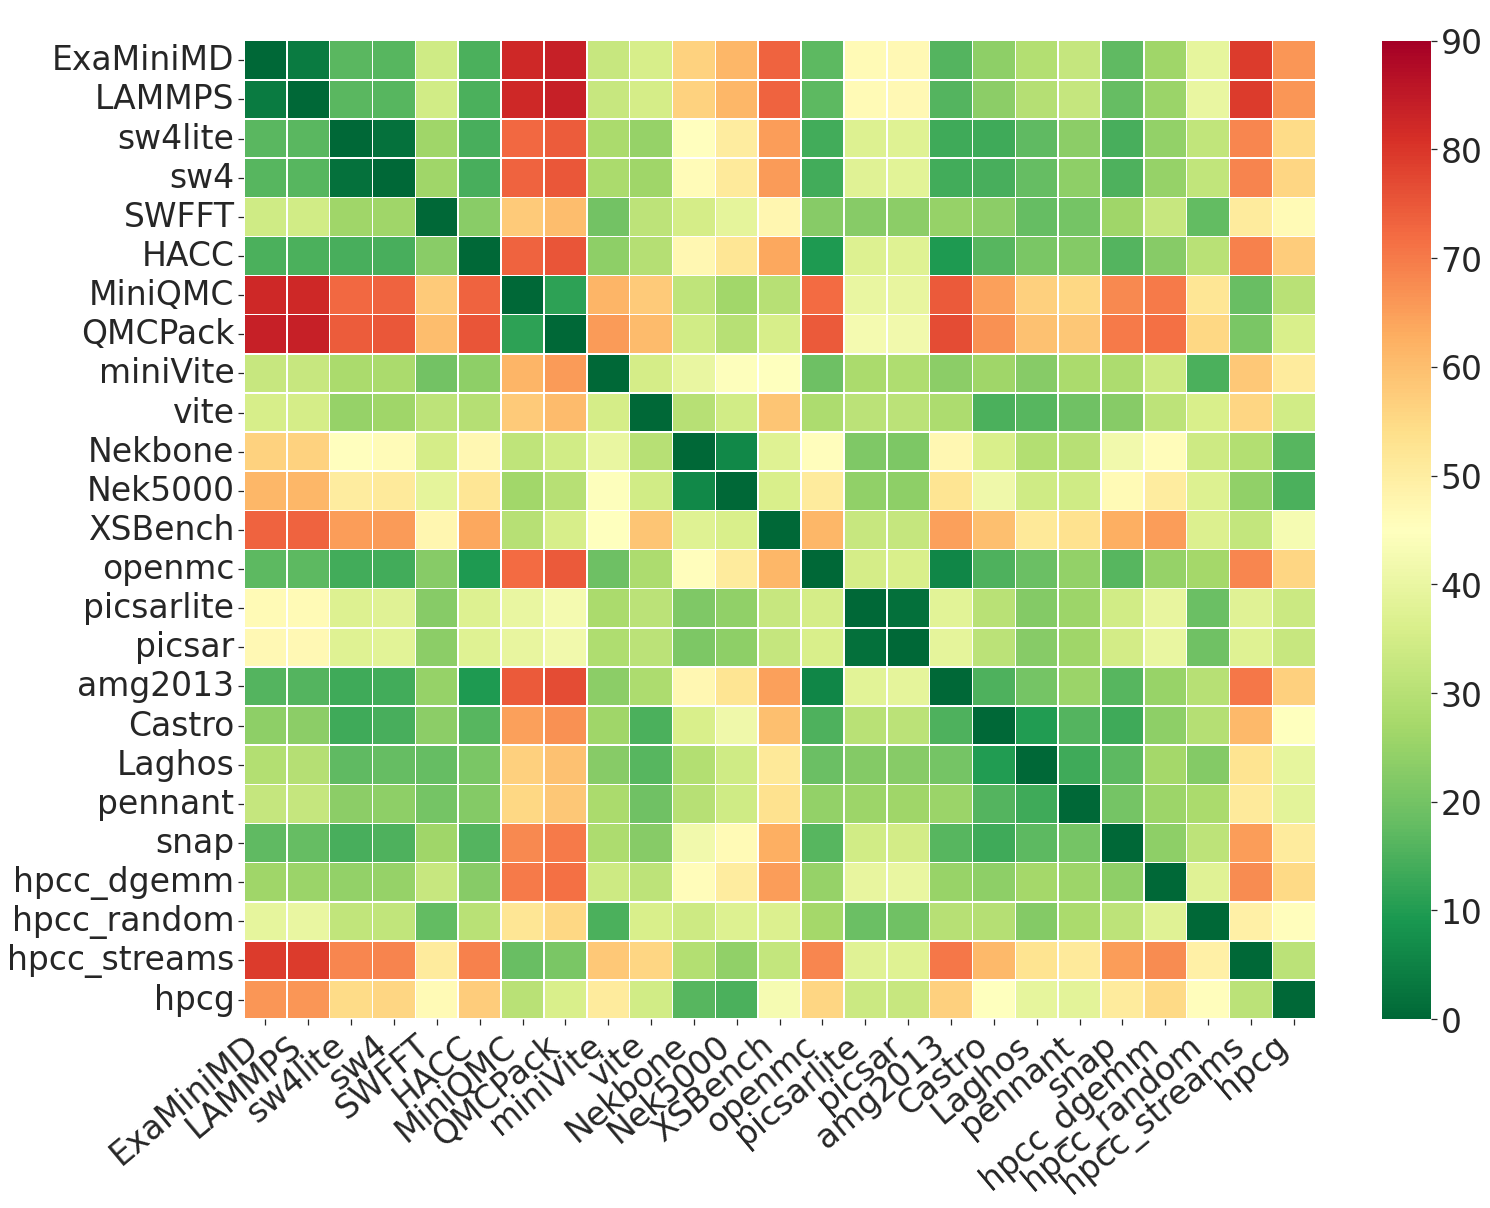
\includegraphics[width=3in]{figs/Cosine_origin_color_nonumber.png}
% 	\vspace*{-5mm}
% 	\caption{Cosine Similarity}
% 	\label{figs:Cosine}
% 	\end{minipage}
% \hspace{.1in}
% \begin{minipage}[t]{0.5\textwidth}
% 	\centering
% 	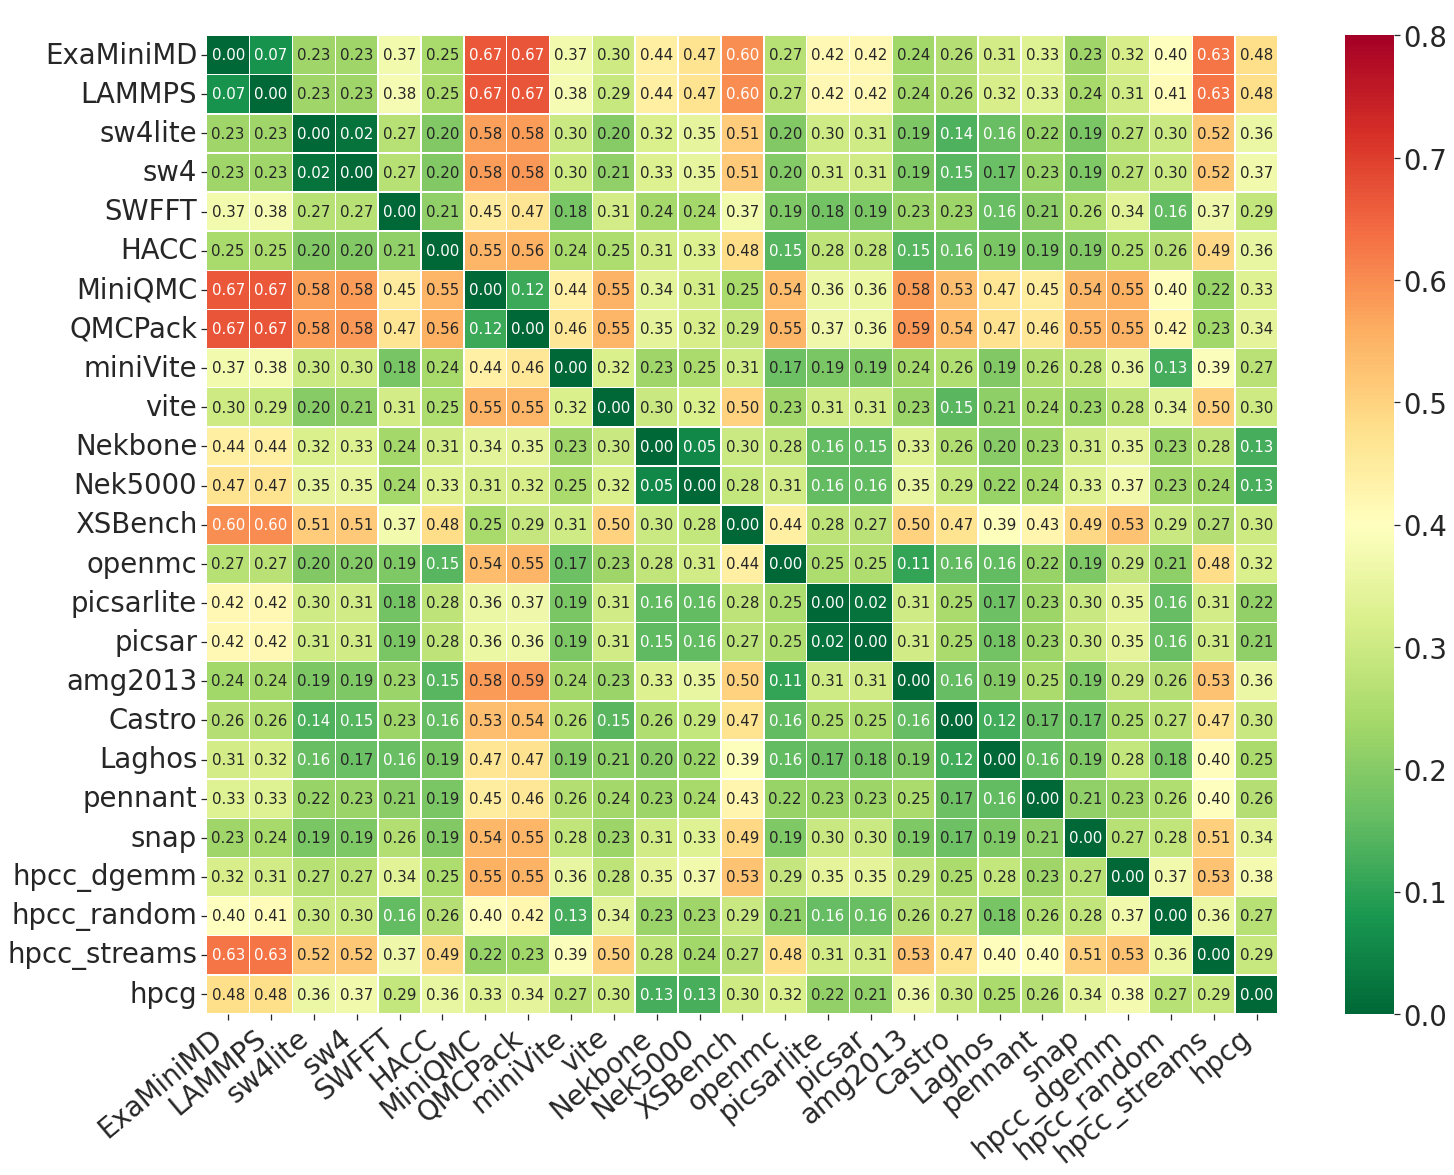
\includegraphics[width=3in]{figs/JS-divergence.png}
% 	\vspace*{-5mm}
% 	\caption{JS divergence}
% 	\label{figs:JS}
% 	\end{minipage}
% \hspace{.1in}
% \begin{minipage}[t]{0.5\textwidth}
% 	\centering
% 	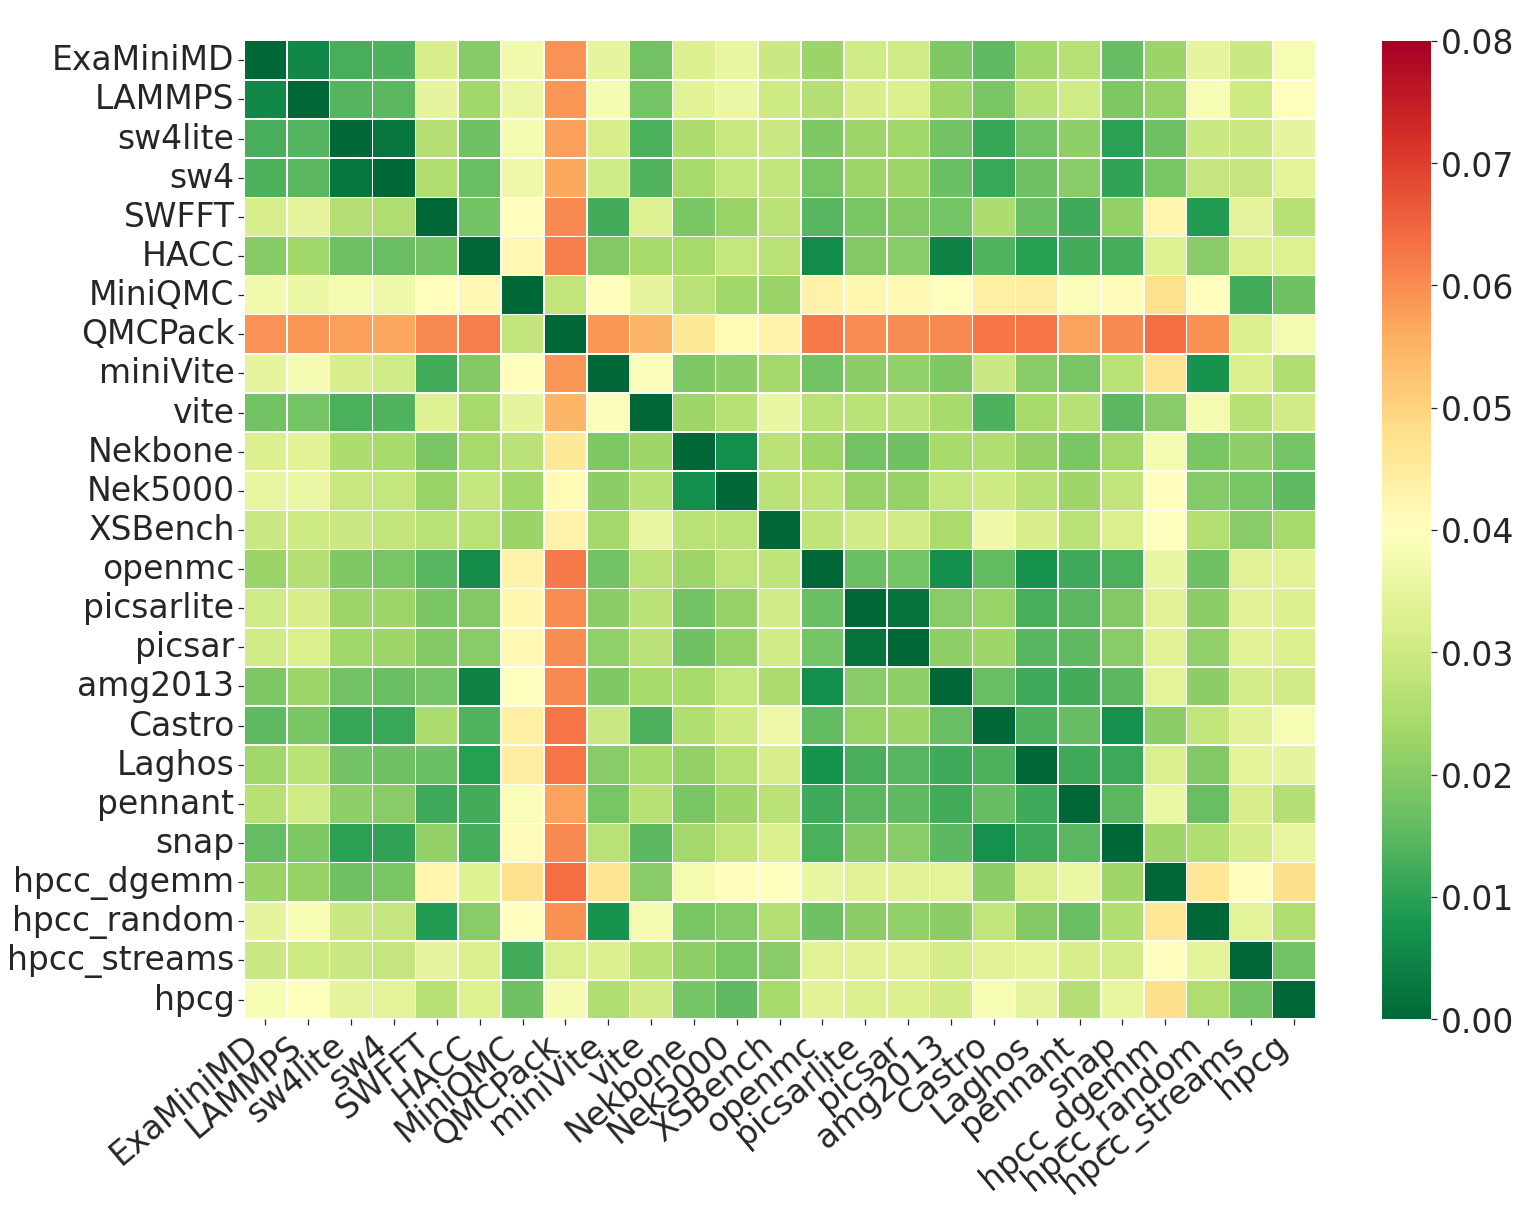
\includegraphics[width=3in]{figs/Wasserstein distance.png}
% 	\vspace*{-5mm}
% 	\caption{Wasserstein distance}
% 	\label{figs:Wasserstein}
% 	\end{minipage}
% \hspace{.1in}	
% \begin{minipage}[t]{0.5\textwidth}
% 	\centering
% 	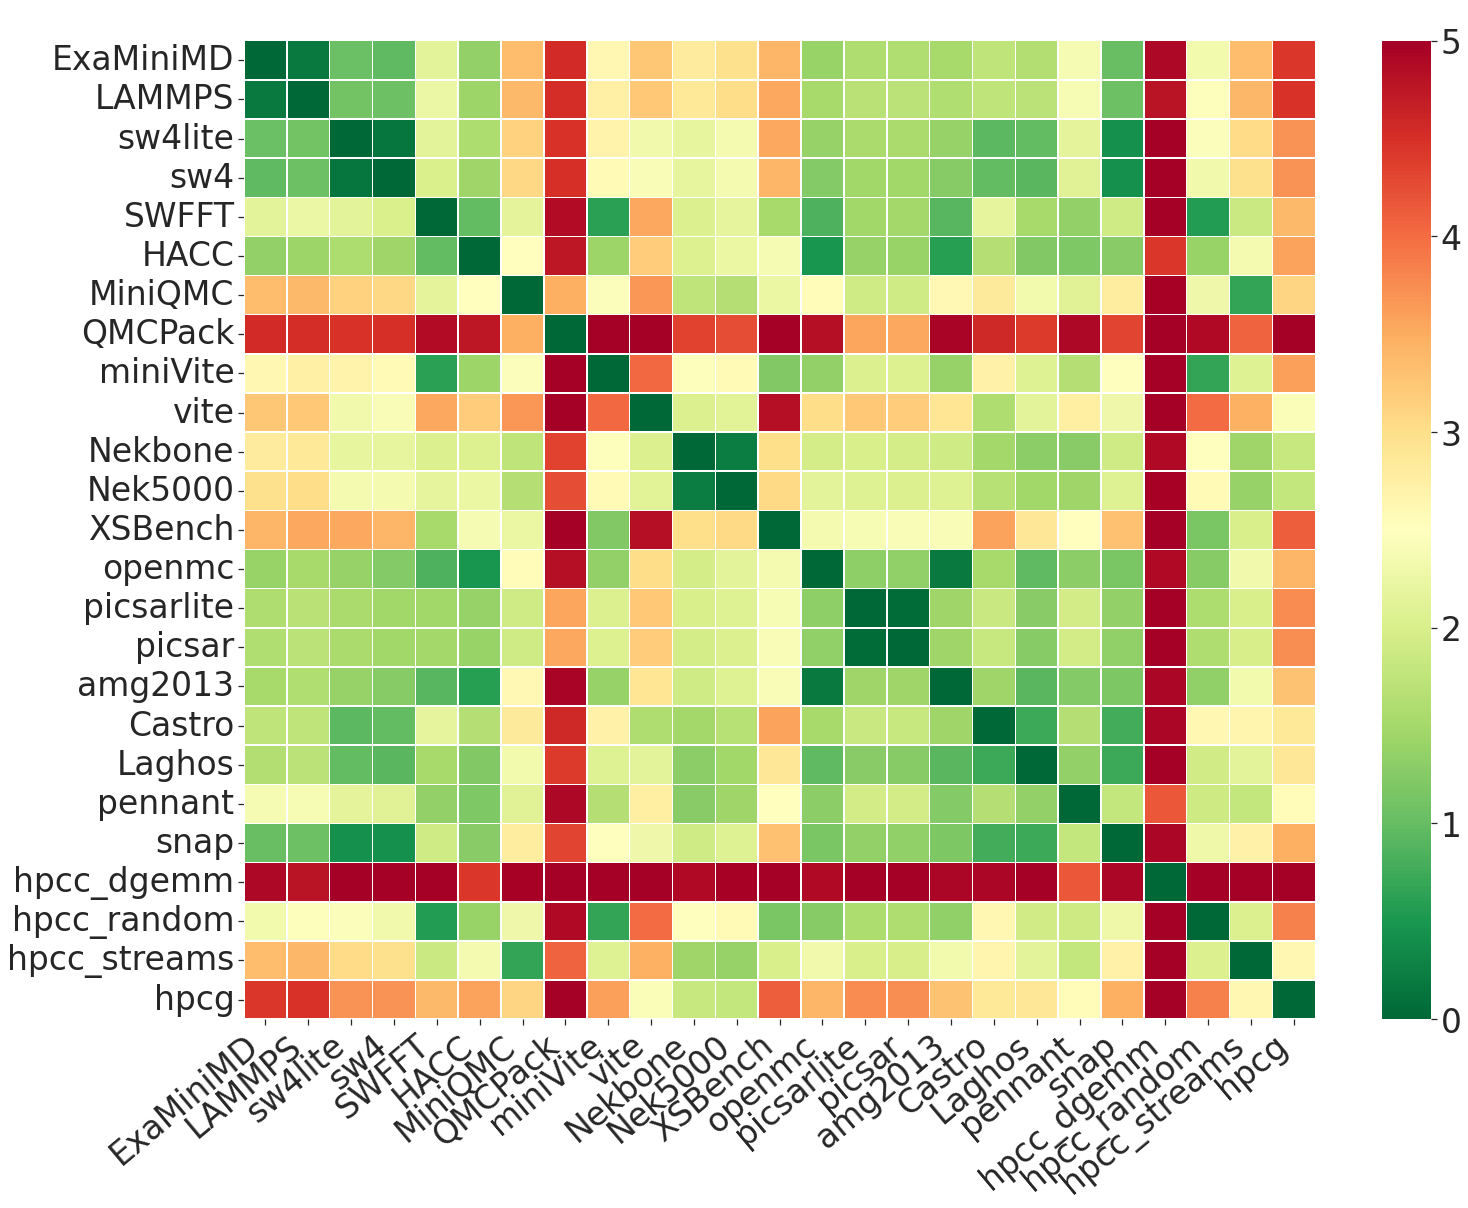
\includegraphics[width=3in]{figs/Mahalanobis distance.png}
% 	\vspace*{-5mm}
% 	\caption{Mahalanobis distance}
% 	\label{figs:Mahalanobis}
% 	\end{minipage}	
% \end{figure}

\begin{figure*}[htbp]
\centering
	\begin{minipage}[t]{0.48\textwidth}
	\centering
	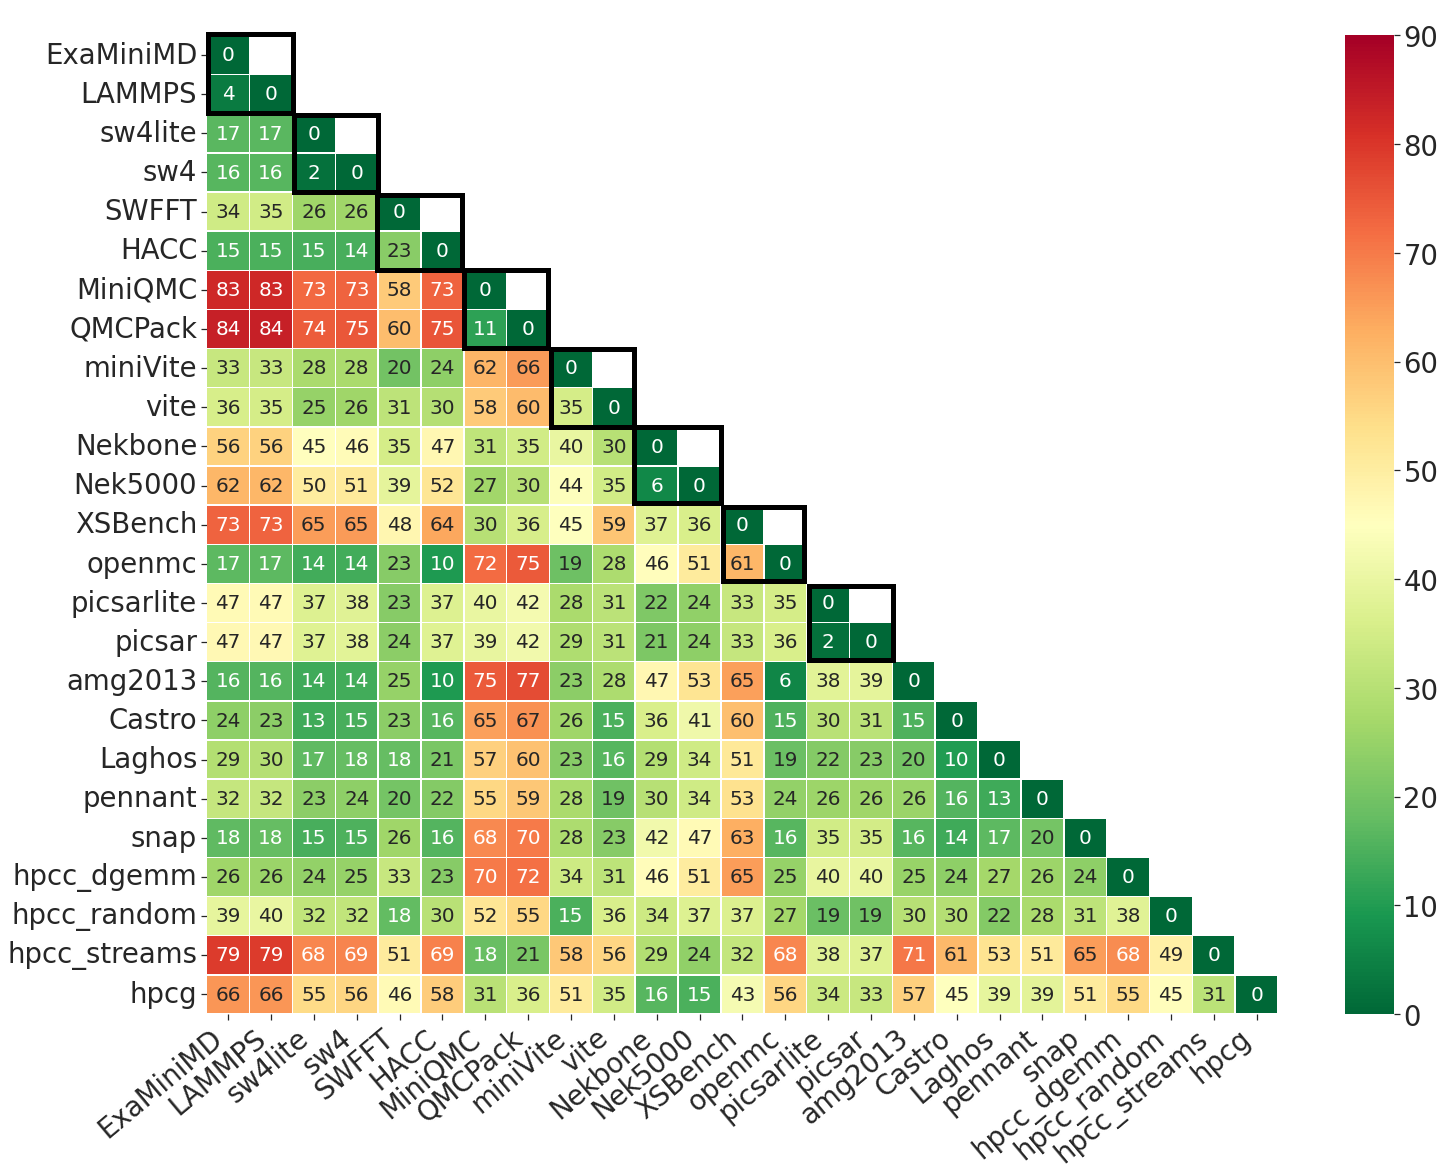
\includegraphics[width=3in]{figs/Cosine_origin_color_tri20.png}
	\vspace*{-5mm}
	\caption{Cosine Similarity}
	\label{figs:Cosine}
	\end{minipage}
\hspace{.1in}
\begin{minipage}[t]{0.48\textwidth}
	\centering
	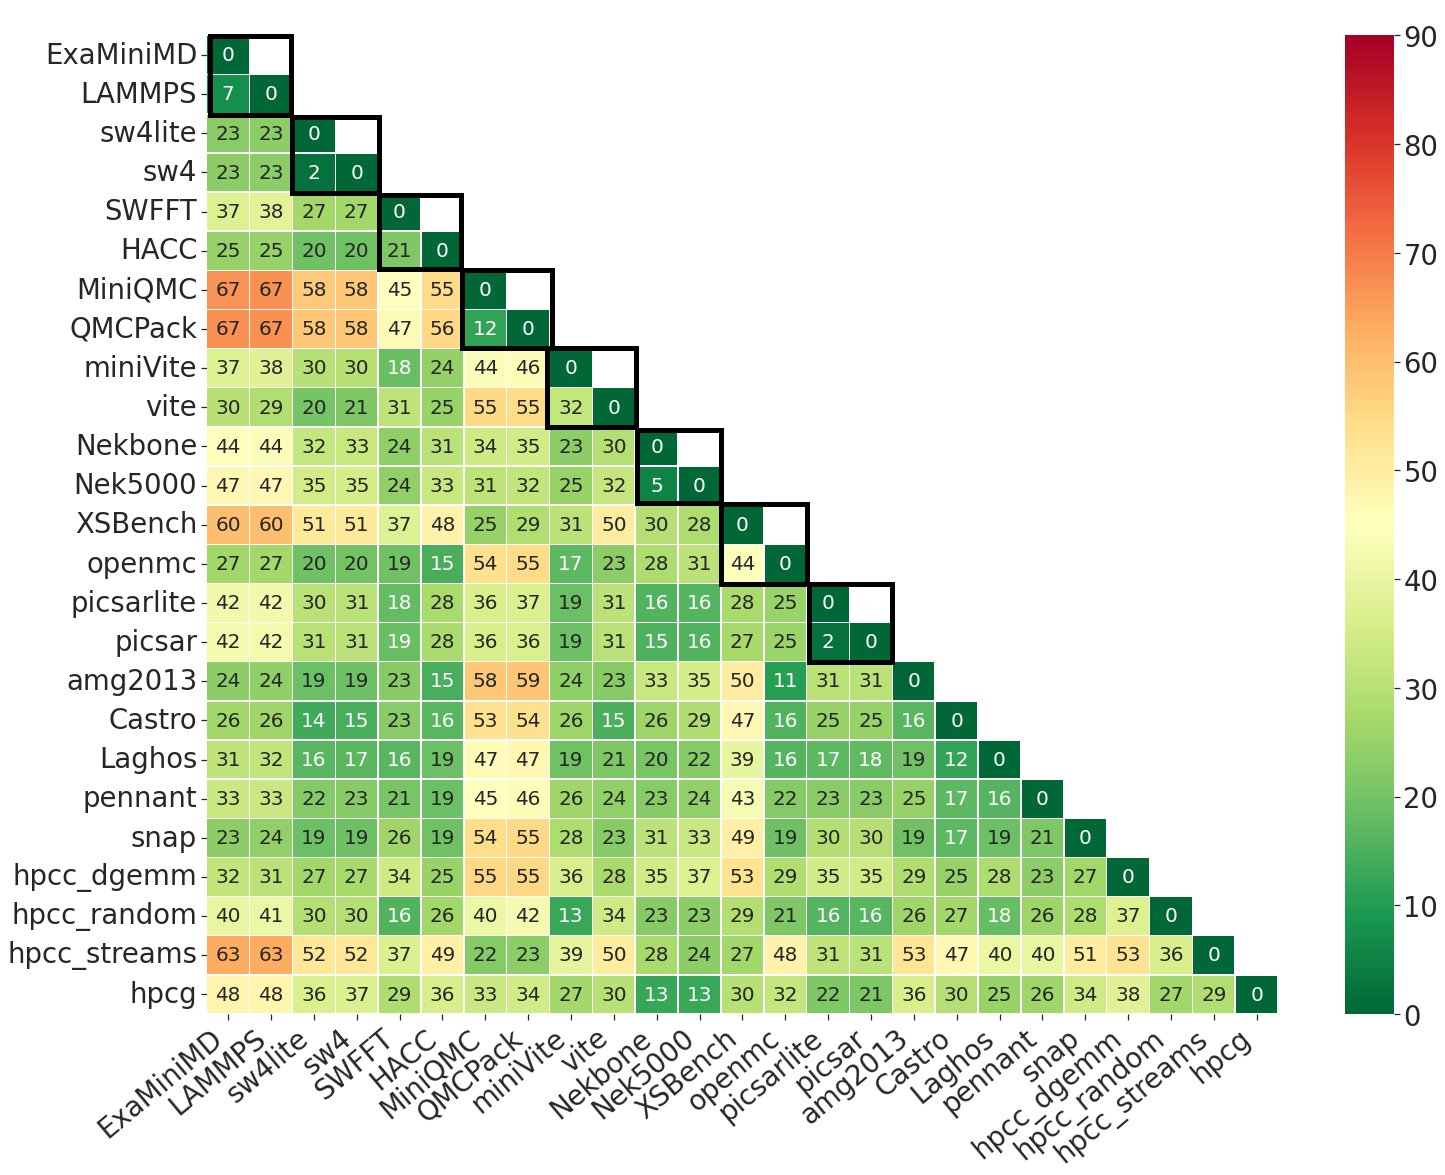
\includegraphics[width=3in]{figs/JS-divergence_m100.png}
	\vspace*{-5mm}
	\caption{JS divergence (Values are multiplied by 100)}
	\label{figs:JS}
	\end{minipage}
\hspace{.1in}
\begin{minipage}[t]{0.48\textwidth}
	\centering
	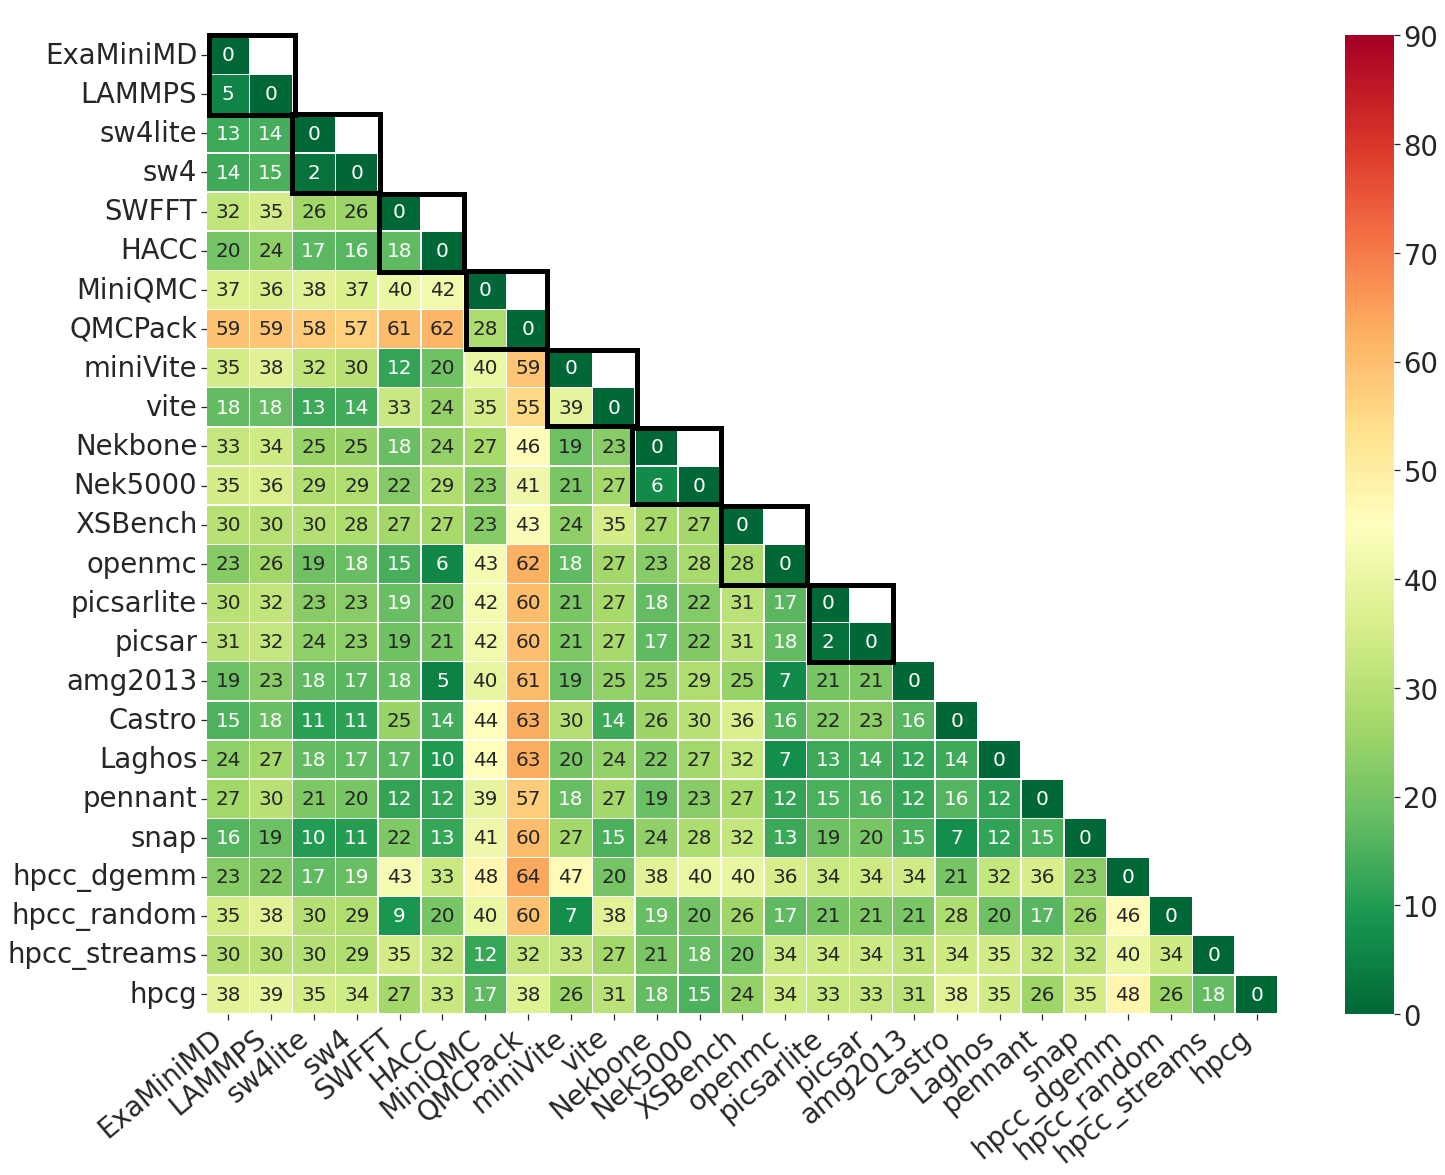
\includegraphics[width=3in]{figs/Wasserstein distance_m1000.png}
	\vspace*{-5mm}
	\caption{Wasserstein distance (Values are multiplied by 1000)}
	\label{figs:Wasserstein}
	\end{minipage}
\hspace{.1in}	
\begin{minipage}[t]{0.48\textwidth}
	\centering
	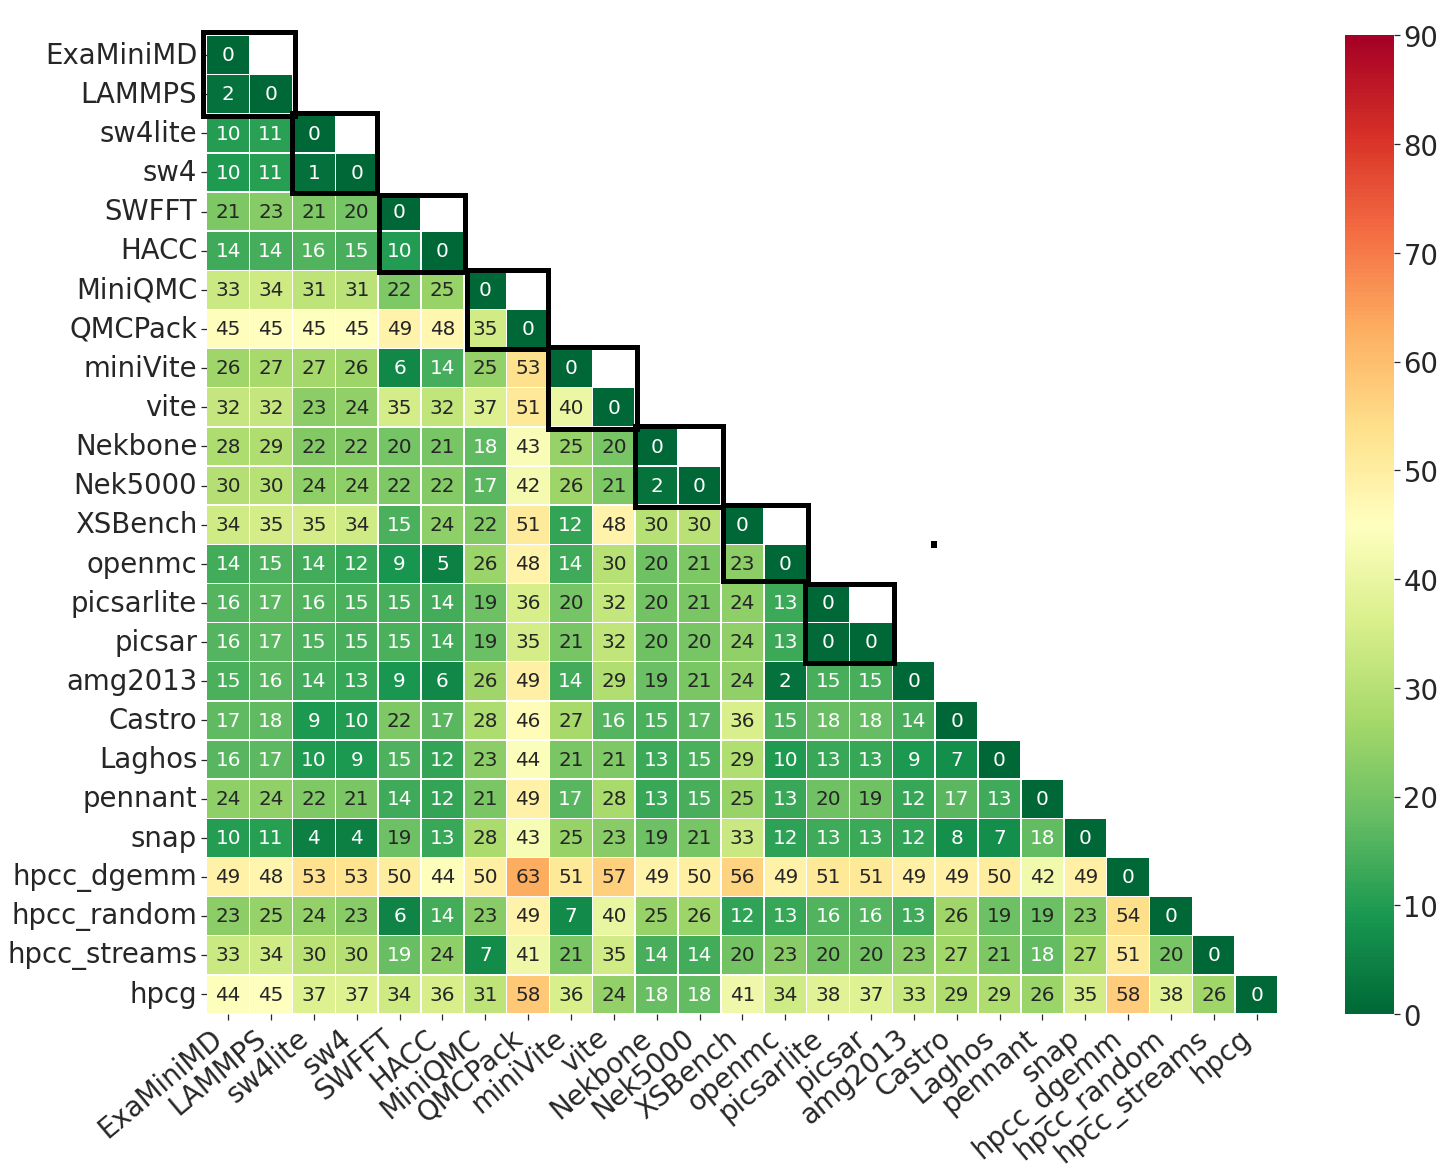
\includegraphics[width=3in]{figs/Mahalanobis distance_m10.png}
	\vspace*{-5mm}
	\caption{Mahalanobis distance (Values are multiplied by 10)}
	\label{figs:Mahalanobis}
	\end{minipage}
\hspace{.1in}
\end{figure*}

Since the similarity matrix is symmetric on the diagonal, we use the lower triangular heatmap to visualize the similarity. The diagonal entries are zero because they indicate the distances between the applications and themselves. We adjust the scale of value in each figure to be the same range to make them comparable. The spectrum colors that represent similarity is from a standard colormap, where dark green is highly similar and dark red is highly dissimilar. All proxies that have parents are listed first on the axes (top on y; left on x) and each parent is listed directly after its corresponding proxy. Along the diagonal, eight 2$\times$2 black border blocks circle the relationship between proxy and parent applications. One would expect to see the lower left of these blocks to be dark green, which show high similarity between proxy and parent. The nine miscellaneous applications (either a proxy with no parent or a parent with no proxy) are listed at the bottom on the y-axis and the right on the x-axis. 

Figures~\ref{figs:Cosine},~\ref{figs:JS},~\ref{figs:Wasserstein}, and~\ref{figs:Mahalanobis} are the overall feature results of four distance methods discussed in Section~\ref{sec:Sim} in the Skylake system. We can see that, generally, the four distance metrics we evaluate return similar correlations. Take for example Figure~\ref{figs:Cosine} which uses cosine similarity, PICSARlite and PICSAR, SW4lite and SW4, Nek5000 and Nekbone, ExaMiniMD and LAMMPS are highly similar proxy/parent application pairs. QMCPack and MiniQMC, and SWFFT and HACC show good similarity.  We get the \textbf{Observation 2}: \textit{75\% of the proxies in our suite demonstrate highly convergent behavior with respect to their parents, and therefore, are faithful representations.} The other two pairs show some behavior gaps. miniVite and Vite are moderately similar. XSBench and OpenMC are highly dissimilar, with an angle of $60^\circ$ between them. This is probably because of the difference in complexity between the parent and proxy in this case; XSBench is only the cross-section lookup portion in Monte Carlo neutron transport, which is a highly data-intensive kernel, whereas OpenMC implements the full neutron transport code so likely has more opportunity to hide poor cache/memory behavior with other computation. The unpaired proxy applications (amg2013, Castro, Laghos, pennant, and snap) used as controls show relative similarity to each other, but do not match the known pairs. The other four HPC benchmark related applications are not similar to each other because they aim to measure total different memory or data patterns. Another thing to note from Figure~\ref{figs:Cosine} is that application pairs QMCPack and MiniQMC are similar to one another, but very different from other applications given lots of red and yellow colors. XSBench, Nekbone, Nek5000, PICSARlite, PICSAR, hpcc\_streams, and hpcg are also outliers in that their behavior shows significant differences compared to most other applications.  It's not surprising that hpcc\_streams is different from other applications because it's a synthetic benchmark program that measures sustainable memory bandwidth and the corresponding computation rate for a simple vector kernel. HPCG is designed to exercise computational and data access patterns that more closely match a different and broad set of important applications. In our suite, only Nekbone and Nek5000 are similar to hpcg.\si{?}

We also notice that there is some diversity when applying these four similarity algorithms. When looking at the dark red areas, applications hpcc\_streams and hpcg are highly dissimilar to other applications in cosine similarity, JS divergence, and Mahalanobis distance, while not that dissimilar in Wasserstein distance. The application hpcc\_degemm is extremely different from other applications in Mahalanobis distance but shows no obvious difference in other similarity algorithms. QMCPack and MiniQMC diverge more in Wasserstein distance and Mahalanobis distance compared to the other two methods, and the difference mainly come from memory and cache subgroup which we will discuss in Sec~\ref{sec:subgroup}. It appears based on ~\cite{qmcpack} that much refactoring effort has gone into QMCPack to improve its memory
behavior and accuracy, and which has not been implemented in miniQMC. We observe that, due to the principle of different similarity algorithms, the diversity of dissimilarity shows different ranges in four distance methods, \eg If the events that have divergent behavior locate far away in the vectors, the Wasserstein distance becomes bigger. Thus, we get the \textbf{Observation 3}: \textit{Similar proxy/parents application pairs remain similar no matter what similarity algorithm is used, while dissimilarities are not the same depending on what algorithm is used.}

Since these distance methods show similar results for similar pairs and the run-time difference of each method is negligible, cosine similarity becomes the preferred similarity metric for our problem due to its simplicity, performance, and ease of interpretability by geometric angle.

\subsection{Important features}
% Laplacian score method requires more sample points for accuracy. Therefore, besides the averaged accumulated data, we also include the original 5 trials' accumulated data. 
Since we assume each application shows similar performance in different trials, and proxy and parent applications show similar performance, we set the parameter of neighbor size to be 2 in the Laplacian score algorithm. After removing the correlated features via the correlation filter, we get 89 ranked features. Table~\ref{tab:top20Cosine} lists the top 20 features, and Figure~\ref{figs:top20Cosine}  shows the cosine similarity matrix using these 20 features. Compared to using all the 500 features as in Figure~\ref{figs:Cosine}, using only the top 20 features can produce more easily graspable similarity information. As we can see in Figure~\ref{figs:top20Cosine}, all 2$\times$2 black border blocks that show high similarity between proxy and parent are preserved. Unsurprisingly, applications that are not pairs remain dissimilar.% the general trend while not the same as the original ones.

\begin{table*}[t]
\caption{Top 20 features}
\label{tab:top20Cosine}
\centering
\begin{tabular}{ll}
\toprule
\small
\textbf{Rank} & \multicolumn{1}{c}{\textbf{Hardware event count names}}            \\ \midrule
1             & `MEM\_LOAD\_UOPS\_L3\_HIT\_RETIRED:XSNP\_NONE'                     \\ 
2             & `OFFCORE\_REQUESTS:DEMAND\_DATA\_RD'                               \\ 
3             & `UOPS\_EXECUTED:THREAD'                                            \\ 
4             & `OFFCORE\_REQUESTS\_OUTSTANDING:ALL\_DATA\_RD'                     \\ 
5             & `OFFCORE\_REQUESTS\_BUFFER:SQ\_FULL'                               \\ 
6             & `MEM\_LOAD\_UOPS\_L3\_MISS\_RETIRED:LOCAL\_DRAM'                   \\ 
7             & `MEM\_LOAD\_UOPS\_RETIRED:HIT\_LFB'                                \\ 
8             & `CYCLE\_ACTIVITY:CYCLES\_L1D\_MISS'                                \\ 
9             & `OFFCORE\_REQUESTS\_OUTSTANDING:ALL\_DATA\_RD\_CYCLES'             \\ 
10            & `CYCLE\_ACTIVITY:CYCLES\_LDM\_PENDING'                             \\ 
11            & `EXE\_ACTIVITY:3\_PORTS\_UTIL'                                     \\ 
12            & `OFFCORE\_REQUESTS\_OUTSTANDING:L3\_MISS\_DEMAND\_DATA\_RD'        \\ 
13            & `BR\_INST\_RETIRED:NEAR\_CALL'                                     \\ 
14            & `OFFCORE\_REQUESTS:ALL\_REQUESTS'                                  \\ 
15            & `ARITH:DIVIDER\_ACTIVE'                                            \\ 
16            & `ICACHE\_64B:IFTAG\_HIT'                                           \\ 
17            & `MEM\_UOPS\_RETIRED:STLB\_MISS\_LOADS'                            \\ 
18            & `OFFCORE\_REQUESTS\_OUTSTANDING:L3\_MISS\_DEMAND\_DATA\_RD\_GE\_6' \\ 
19            & `UOPS\_DISPATCHED:PORT\_1'                                         \\ 
20            & `MEM\_UOPS\_RETIRED:SPLIT\_STORES'                                 \\ \bottomrule
\end{tabular}
\normalsize
\end{table*}

\begin{figure}[ht]
\centering
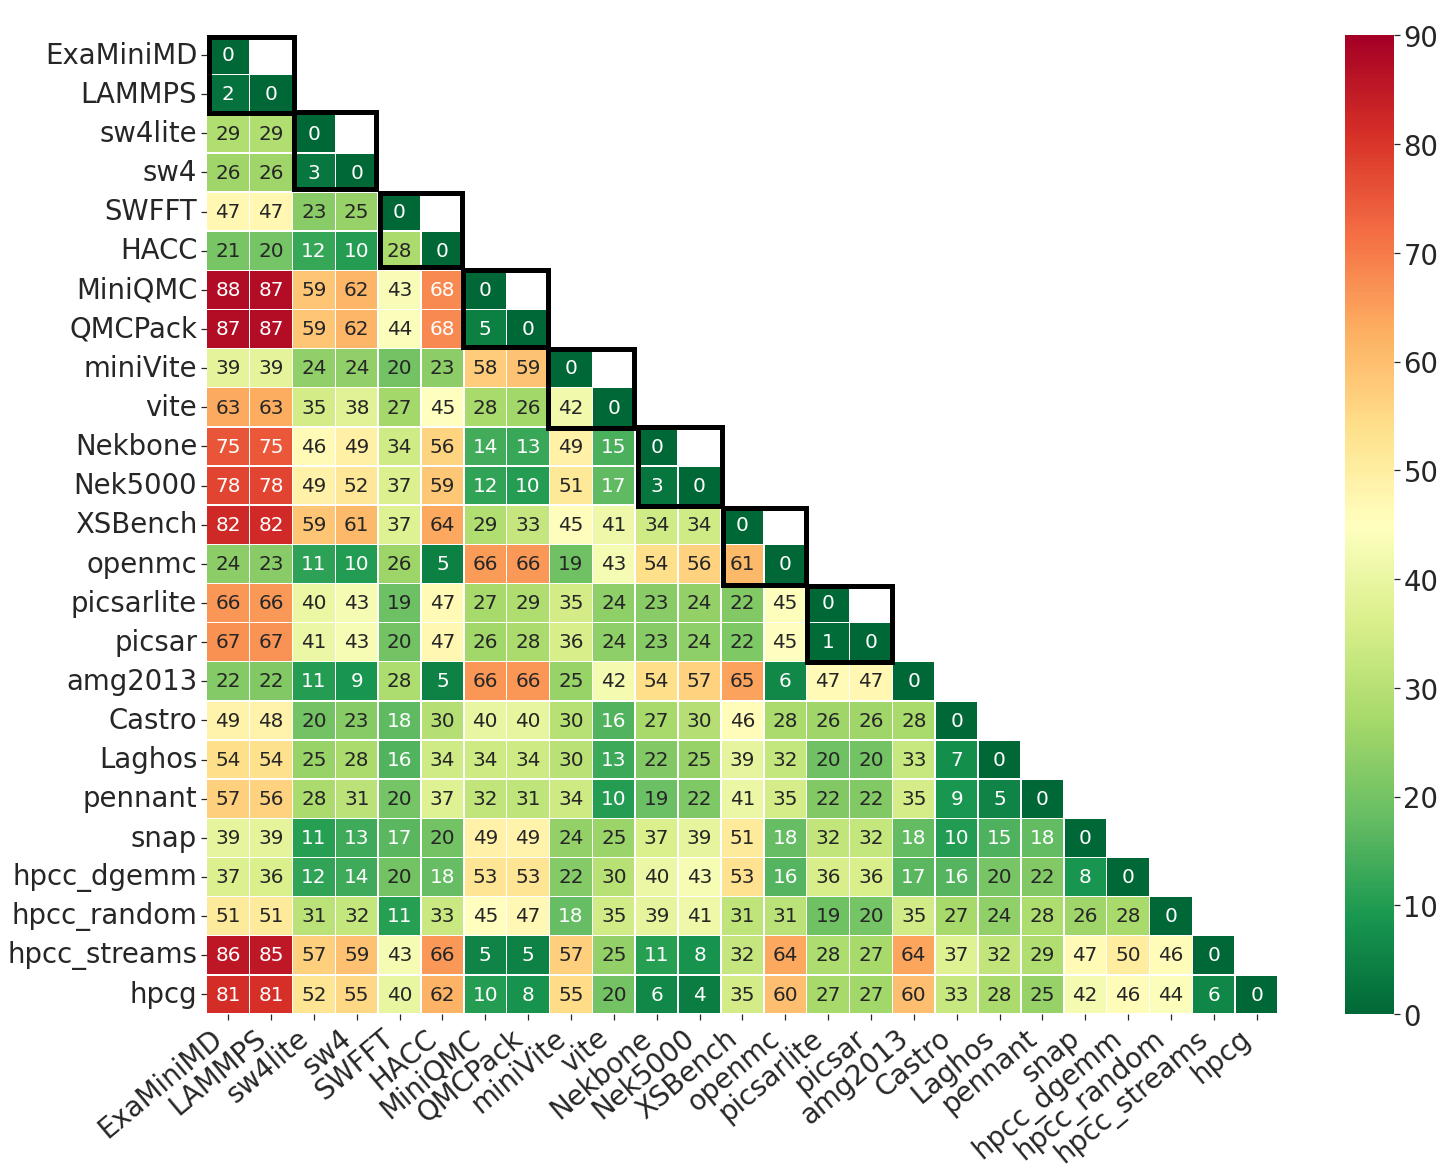
\includegraphics[width=\linewidth]{figs/top20cosine_origin_color_font20.png}
\caption{Cosine Similarity with top 20 important features}
\label{figs:top20Cosine}
\end{figure}

\subsection{Feature Standard Deviation}
\label{sec:Dev}
Besides selecting the important features to preserve the similarity of proxy and parent pairs, we are also curious about what contributes to the dissimilarity of the proxy and parent pairs. Therefore, we investigate the run-time time series. Using the data of hardware event counts per second, we get the standard deviation for each application on each feature (hardware event counts). If one point is located within 2 standard deviations, we consider this point to be within the distribution.


We calculate the standard deviation of each feature for each parent application and check whether the accumulated mean of the according feature of a proxy application is within two standard deviations of the parents' accumulated mean within a normal distribution. 
Table~\ref{tab:Dissimilarity} shows the feature numbers for each proxy/parent pair when the difference is bigger than 2, 3, 4, 5 standard deviations separately. The result is as we expected as in Figure~\ref{figs:Cosine}. We can see that SW4lite and SW4, and PISCARlite and PISCAR, are the most similar proxy/parent pairs because, in each pair, the proxy only has one feature (`MOVE\_ELIMINATION: SIMD\_NOT\_ELIMINATED' and `UOPS\_EXECUTED: X87' separately) deviate relatively far from the parent. The proxies that have more features deviating farther from their parents are accordingly less similar. \eg miniVite and Vite have 72 features with large deviation, and they are moderately similar with 35 degrees in the cosine similarity matrix Figure~\ref{figs:Cosine}. This 
brings us \textbf{Observation 4}: \textit{A proxy application that has most of the hardware event counts within standard deviations of the parent application is similar to its parent.} 



\begin{table}[t]
\caption{Dissimilarity feature source for proxy/parents pairs}
\label{tab:Dissimilarity}
\centering
\begin{tabular}{lrrrr}%llll}
\toprule
\textbf{Proxy and Parent pairs}               & \textbf{\textgreater{}2std} & \textbf{\textgreater{}3std} & \textbf{\textgreater{}4std} & \textbf{\textgreater{}5std} \\ \midrule
ExaMiniMD / LAMMPS                            & 10                          & 8                           & 8                           & 4                           \\ 
SW4lite / SW4                                 & 1                           & 1                           & 1                           & 1                           \\ 
SWFFT / HACC                                  & 17                          & 12                          & 11                          & 8                           \\ 
miniQMC / QMCPACK                             & 13                          & 10                          & 8                           & 6                           \\ 
miniVite / Vite                               & 72                          & 38                          & 23                          & 21                          \\ 
Nekbone / Nek5000                             & 11                          & 6                           & 2                           & 2                           \\ 
XSbench OpenMC                                & 16                          & 9                           & 9                           & 8                           \\ 
PICSARlite / PICSAR                           & 1                           & 1                           & 1                           & 0                           \\ 
Unique feature \#s & 99                          & 64                          & 49                          & 38                          \\ \bottomrule
\end{tabular}

\end{table}


\subsection{Subgroup Features}
\label{sec:subgroup}
In addition to studying the features overall, we also investigate the similarity in subgroups, since we collect the data in subgroups as in Sec \ref{sec:collect}. We could focus on a subgroup behavior that we are interested in, instead of considering them overall. 
For example, if one is using this data to choose proxy applications for a memory study, memory behavior diversity can have a much larger impact on the choice. In contrast, if one is using this data to decide if a proxy can be used to examine refactoring code for improved memory performance, a small difference between proxy and parent in memory may not matter. 

We look at many subgroups of data. Some subgroup matrices have no colors other than green or light green (no dissimilarity), while others show the applications which are outliers in those subgroups. Here we show some matrices that have extensive dissimilarities. Figure~\ref{figs:cosine L1_D_Cache} shows similarity over only L1 cache related performance counters. We can see that applications MiniQMC and QMAPack are relatively
similar to each other but dissimilar to others in this subgroup. In the memory pipeline subgroup (Figure~\ref{figs:cosine Memory_Pipeline}), ExaMiniMD and LAMMPS show dissimilarity to others. In the Execution Pipeline subgroup (Figure~\ref{figs:cosine Execution_Pipeline}), MiniQMC, QMAPack, XSBench, hpcc\_streams have divergent behavior from all
other applications.
We cannot describe all examples in this paper, but the investigation in subgroups gives us a way to see similarities in specific fields.\avani{can we add this to an appendix?} \si{appendix counts in pages}

\begin{figure}[ht]
\centering
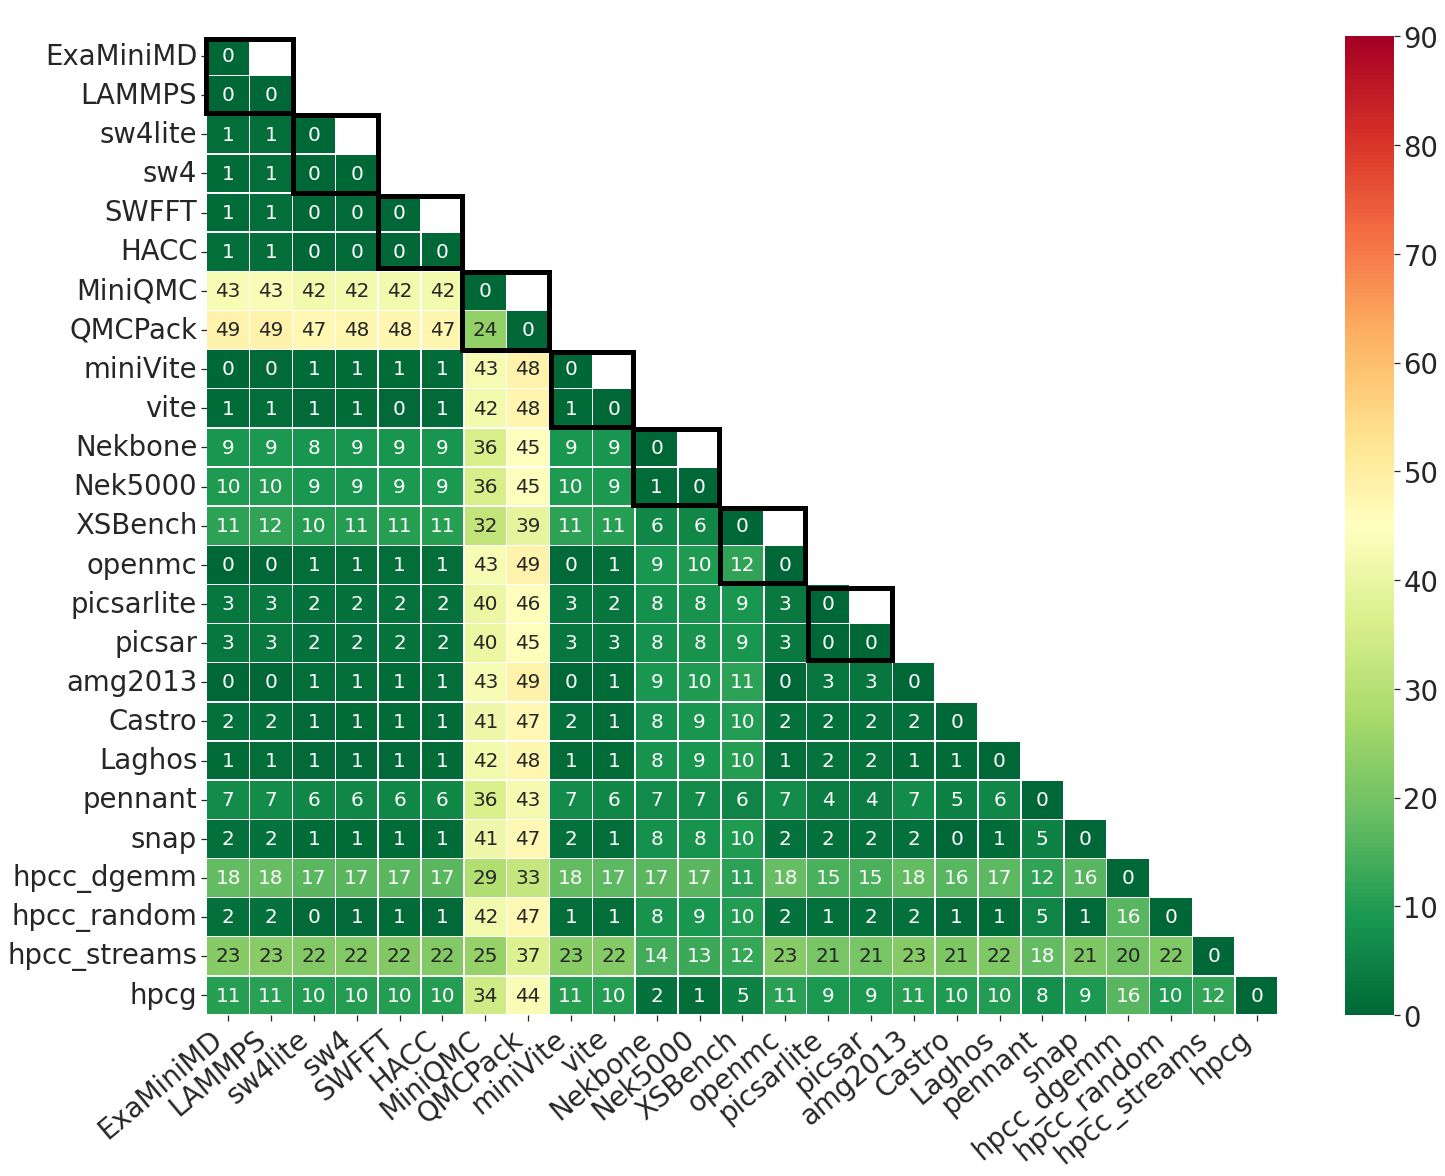
\includegraphics[width=0.9\linewidth]{figs/L1_Cache_font20.png}
\caption{Cosine Similarity for L1 Cache }
\label{figs:cosine L1_D_Cache}
\end{figure}

\begin{figure}[ht]
\centering
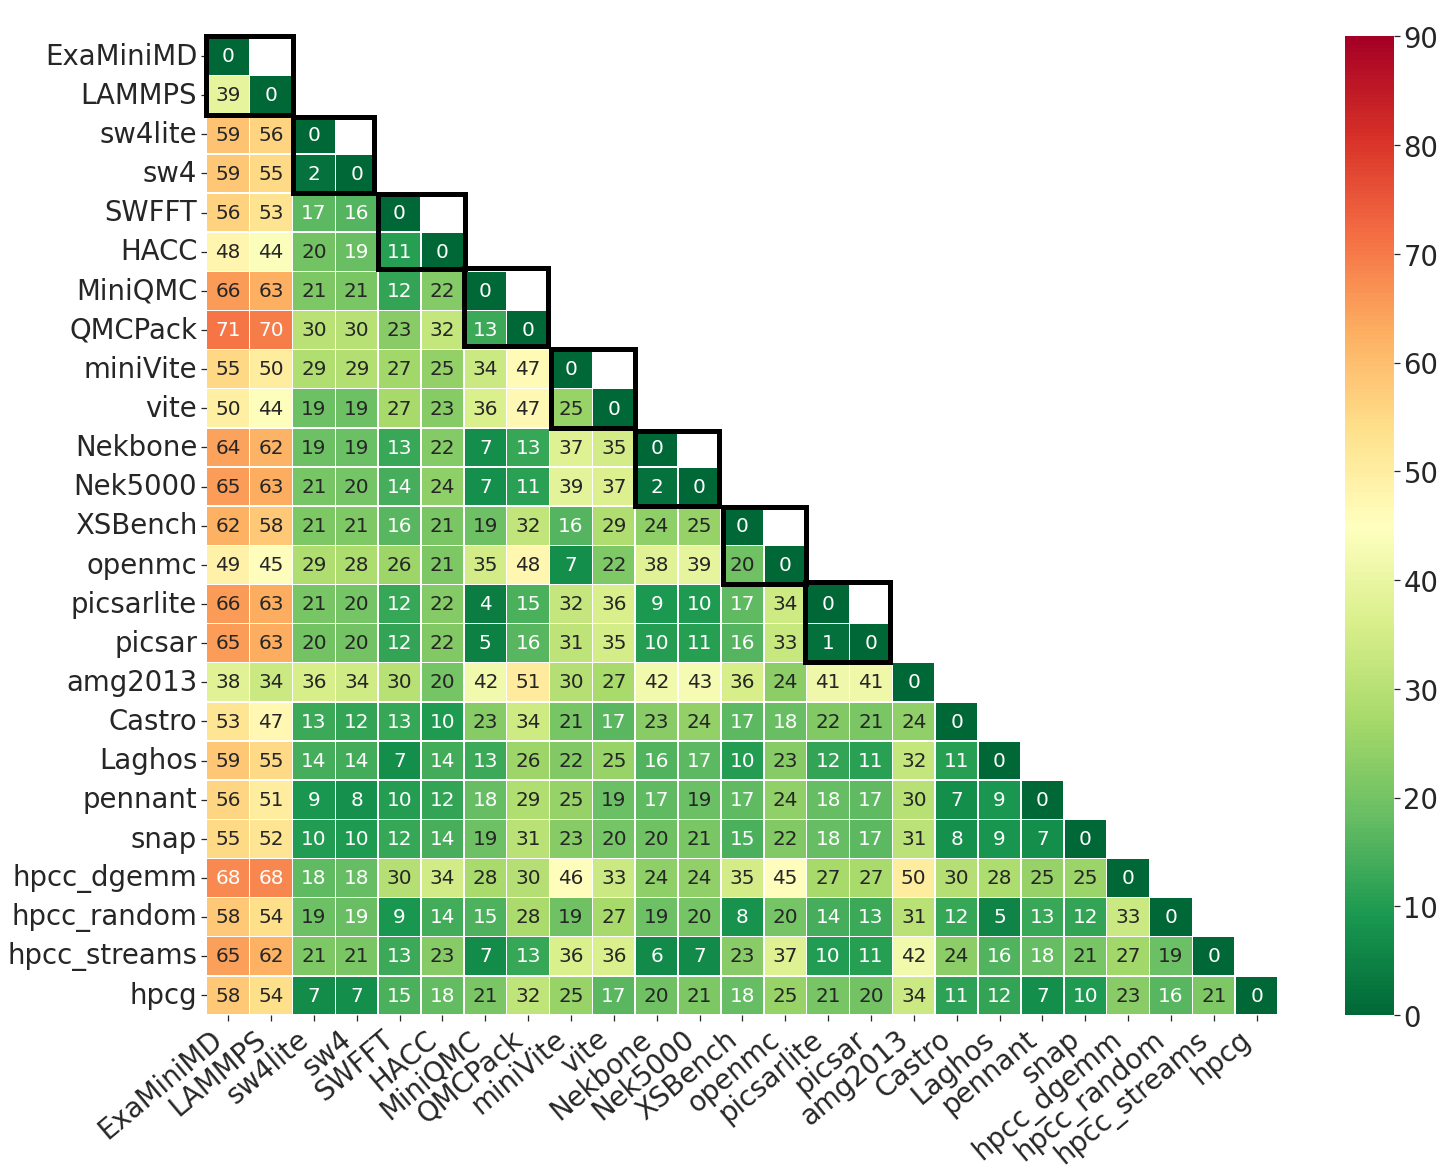
\includegraphics[width=0.9\linewidth]{figs/Memory_Pipeline.png}
\caption{Cosine Similarity for Memory Pipeline }
\label{figs:cosine Memory_Pipeline}
\end{figure}

\begin{figure}[ht]
\centering
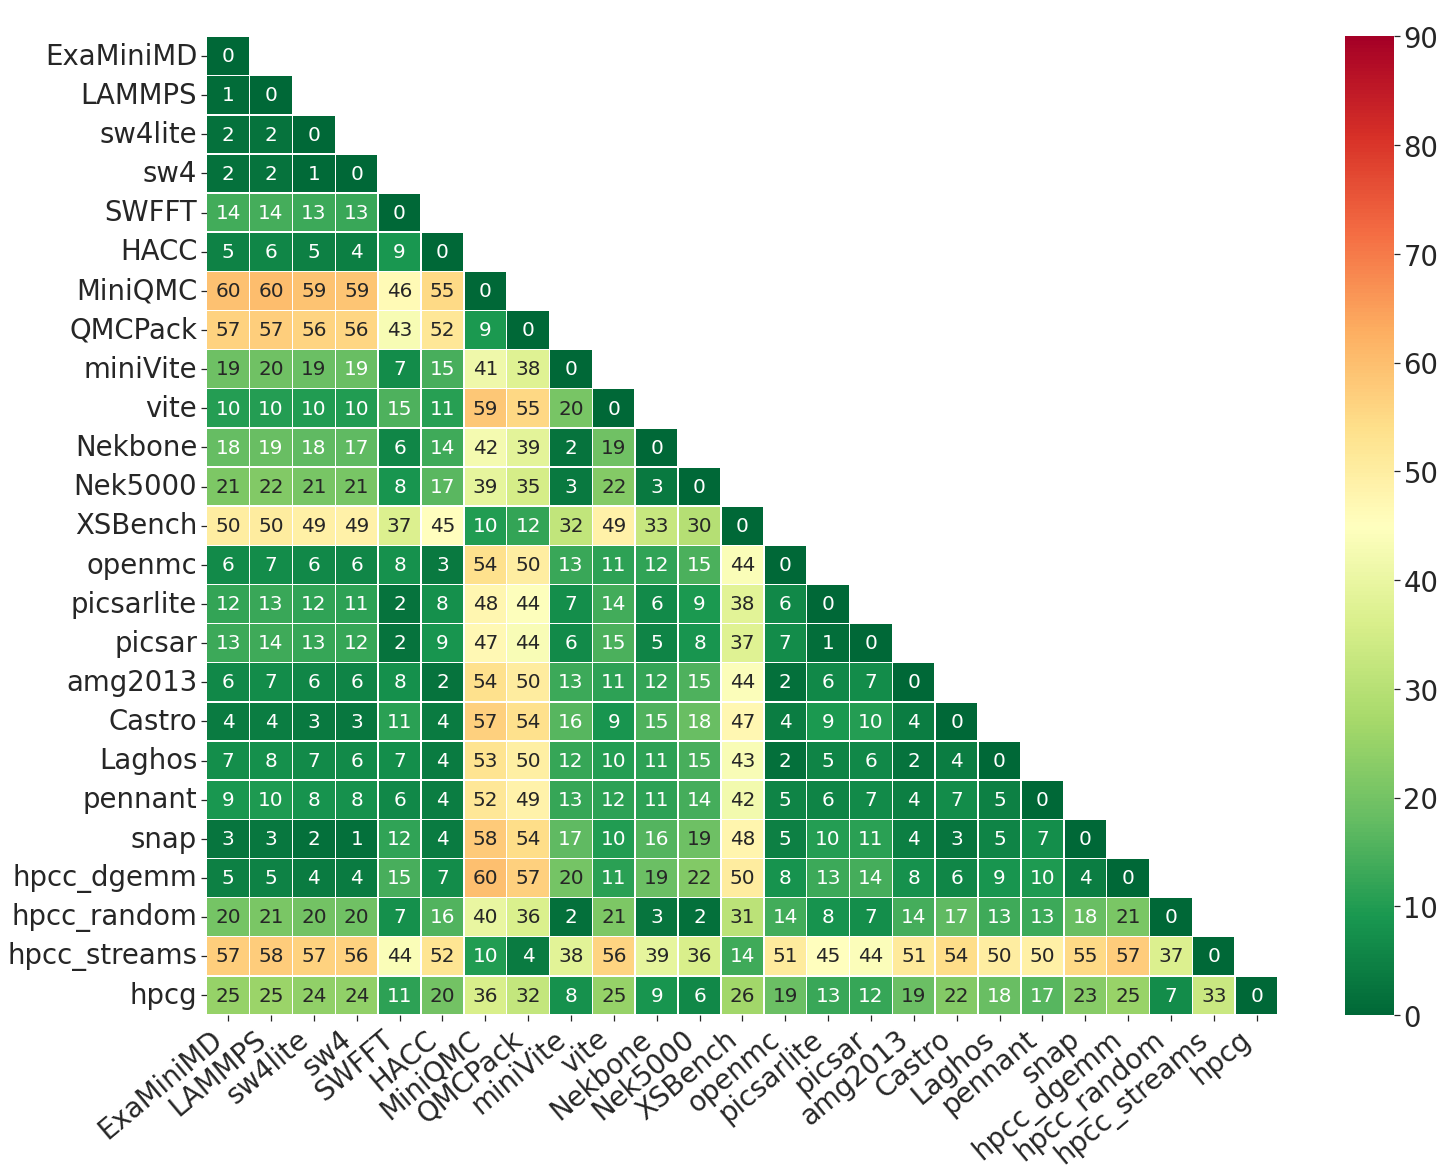
\includegraphics[width=0.9\linewidth]{figs/Execution_Pipeline.png}
\caption{Cosine Similarity for Execution Pipeline }
\label{figs:cosine Execution_Pipeline}
\end{figure}


\subsection{Discussion}
\avani{to expand}
%\si{shall we move this to discussion?}
%Notice that to collect the complete set of data, we run each application multiple times. Run-time variance is inevitable among multiple runs. Therefore, when we combine all the features if we want to keep the time phases, we need to consider aligned data. The run-time differences also occur among different applications, \eg most parent applications have longer run-time than corresponding proxy applications. Since our current analysis is based on the final accumulated average of each hardware event counts for each application, we temporarily do not take the run-time differences into account. For future work of time phases comparison, we have implemented run-time alignment for each application with a weighted index for each run. 
Our results indicate, surprisingly, that the particularities of the similarity algorithms have less impact than predicted on the likelihood of correlating parent/proxy pairs.  Since we use ECP pairs, we expect that this is a general result, but we cannot rule out the possibility that some domains will not have clearly separable parent/proxy relationships.

Run-time variance is inevitable in HPC. On the one hand, to collect the complete set of data, we run each application multiple times. Minor run-time differences occur among multiple runs. On the other hand, different applications vary in run-time, \eg most parent applications have longer run-time than their corresponding proxy applications. Since our current analysis is based on the final accumulated average of each hardware event count for each application, we temporarily do not take these run-time differences into account. However, if we want to keep the time phases for each application, we need to consider aligned data. Currently, we have implemented run-time alignment for each application with a weighted index for each run, but aligned data could be used for future time phase comparison. 

For future work, we will evaluate the important features on more platforms. Since currently our analysis is based on the final accumulated average of each hardware event counts, the variance of run time for each application is negligible after we average the results. Therefore, we do not take time phases into account. Recently, We have implemented run-time alignment for each application. For the next step, we will analyze the time phases across proxy/parent application pairs.

\todo{List / expand upon other places this could be used: compiler studies, to understand what's different when refactoring applications}  \jeanine{todo}
\section{Related Work}
\label{sec:relatedWork}
\subsection{Proxy Application Characterization}
Proxy application characterization, including the comparison of individual proxies to their parent applications~\cite{BARRETT2015107, Islam:2016:MLF:3014904.3014966, 8049024, CPE:CPE3587} and performance projection~\cite{barrett2012navigating, sharkawi2009performance,8049025} have been well studied. We present the most recent related work below. 

Aaziz et al.~\cite{8514880} applied hierarchical clustering to a small selected subset of hardware performance event counters across proxy/parent pairs to understand behavior similarity at the node level. Although this method accurately clusters proxy/parent pairs that are similar, it provides more of a relative measure of similarity between similar proxy/parent pairs.  The similarity is measured by tree branch height, which has little physical
meaning. Additionally, this method did not provide a visual representation that enabled a quick understanding of the range of application behavior represented (or not) by the suite of proxy applications used. Therefore, eliminating proxies with redundant behavior was not easily supported by this method.

Tramm et al. ~\cite{XSBench} perform a characterization of OpenMC, and its proxy, XSBench. Multi-core scaling efficiency, floating point calculation rates, and hardware performance counter profiles are correlated to an efficiency loss metric that is related to performance as the number of threads is increased.  This work is a study on a single proxy/parent application pair and presents a methodology that is manual rather than machine-learning based. They focus more on the characterization of performance, particularly for proxies, and they present similarity of proxies, rather than similarity of proxy/parent pairs.  Kim et al.~\cite{8049024} extend their KGen Fortran Kernel Generator tool with the ability to gather descriptive statistics from both the original application and the KGen kernel extracted from the instrumented application. They do not evaluate proxies, but rather extract a kernel from an application, and apply general descriptive statistics.

Barrett et al.~\cite{BARRETT2015107,CPE:CPE3587} are active in developing proxy applications and in assessing their characteristics with real applications. In~\cite{CPE:CPE3587} they do an in-depth analysis of one real and proxy application pair (Charon/miniFE), while in~\cite{BARRETT2015107} they propose a methodology whereby a set of performance domains is considered for some pair of proxy and real applications, and comparison and threshold functions are created for each performance domain.  For example, for the LAMMPS/miniMD pair (molecular dynamics), their domains are total time, force calculation time, neighbor list construction time, and inter-process communication time. While the abstract methodology framework is common, since the instantiation for each pair of applications is unique, their work is somewhat orthogonal to ours, as we are proposing a common instantiated methodology.

Islam et al. ~\cite{Islam:2016:MLF:3014904.3014966} created the Veritas framework to measure proxy/parent relationships using belief estimation in Dempster-Shafer theory over low level resource measurements of CPU component usage. They then computed the amount that a proxy \emph{covers} the real application in each of the resource categories. The resource categories they used were floating point, branch execution, TLB, L1-L3 caches, memory, and prefetching. They also used PCA to achieve some dimensionality reduction in their data.

Tsuji et al.~\cite{8049025} address the use of proxy applications to inform the use of benchmark applications as a precursor in assessing expected system performance. They propose a new metric, SSSP or Simplified Sustained System Performance, based on a prior SSP method and calculated over kernel benchmarks rather than real applications. This adapted methodology avoids the use of real applications in establishing system performance, which is known to be costly to set up and tune to a given system. They demonstrate the consistency of SSSP with SSP while only utilizing data from proxy applications and simple benchmark kernels. A similar form of performance projection is likewise presented by Sharkawi et al.~\cite{sharkawi2009performance}. Dickson et al.~\cite{7836562} extract an I/O pattern from an application and recreate that pattern in a proxy application which is used to explore alternative I/O library paradigms. This work is specific to I/O behavior and does not evaluate existing proxies, but is valuable since existing proxies often ignore I/O behavior.

%Aaziz et al.~\cite{aaziz2018methodology} applied hierarchical clustering to a small selected subset of hardware performance event counters across proxy/parent pairs to understand behavior similarity at the node level.
\subsection{Distance Metrics and Feature Selection}
Other cosine similarity metrics including Square Root Cosine Similarity and Improved Square Root Cosine Similarity have also been studied in ~\cite{sohangir2017improved}, however, neither reflects identity in the case of comparing a vector with itself nor does either present a clear geometric understanding of the comparison. There are more similarity algorithms available, but not included in this paper. Our work serves as a metaanalysis across similarity methods, demonstrating their interchangeability in this domain. 

Distance metric learning is a branch of machine learning that aims to learn distances from
the data, which enhances the performance of similarity-based algorithms~\cite{suarez2021tutorial}. Automatically learning customized metrics from data~\cite{bellet2013survey} has attracted a lot o interest in recent years. \eg given some examples of similar pairs of points, a linear transformation matrix (Mahalanobis distance metric) is learned to represent these relationships~\cite{xing2002distance,weinberger2009distance}. However, these approaches have an assumption that similarity or dissimilarity is clearly defined, while in our problem this is not the case.


Most existing unsupervised feature selection algorithms such as Relief~\cite{kira1992practical} and ReliefF~\cite{kononenko1997overcoming}, Laplacian score~\cite{he2005laplacian}, Fisher Score~\cite{jennrich1976newton}, SPEC~\cite{nguyen2014effective}, HSIC~\cite{yamada2012high}, and Trace Ratio~\cite{nie2008trace}, are essentially based on assessing features' capability in preserving similarity. However, a common drawback is being unable to handle feature redundancy~\cite{zhao2011similarity}. In Lindenbaum \etal~\cite{lindenbaum2021differentiable}, nuisance features are filtered before computation of importance to improve the accuracy and efficiency. Yu \etal~\cite{yu2003feature} proposes a correlation-based filter to remove the redundancy in a supervised scenario.
PFA~\cite{lu2007feature} exploits the structure of the principal components by choosing the important features with the nearest distance to the cluster center, but the assumption of normalized distribution for k-means may not be true in some circumstances. Li \etal~\cite{li2018feature} reviews some feature selection algorithms for structured data where features exhibit group, tree, or graph structures, but most of them need prior knowledge of structures, which is still a challenging problem for automatic feature selection.

\section{Conclusion}
\label{sec:conclusion}
We have evaluated different similarity metrics to determine the fidelity of proxy applications with respect to their corresponding parent applications.
%
We show that most proxies are faithful representations of their parents, with minor divergences, independent of the similarity metric used.  Thus, we demonstrate that efficient, low-overhead metrics such as cosine similarity are sufficient for proxy evaluation.
%
We propose a feature selection framework called \us to find the most representative features, which efficiently shows the critical features in evaluating the similarity for proxy and parent pairs while greatly decreasing the data collection overhead. 
%
We demonstrate that the selected concise feature set captures the similarities across applications.
%
As well, we show some features that identify the dissimilarity between proxy and parents pairs, which would help the proxy co-design in the long run.
%
Similarity measurement and feature selection approaches in \us can also be applied to various HPC problems, such as compiler optimization, code refactoring, and application input sensitivity.
\todo{End on broad notes; mention again how this is important to HPC / other domains}
\todo{Make certain post-reference dangling figures are addressed before submission}
\commentout{ %---anonymous submission-----
\section{Acknowledgment}
}


\section{lock}
owner,file










\bibliographystyle{abbrv}
\bibliography{ref}

\begin{appendices}
\appendix
\appendixpage
\section{Additional Data}
\label{appendix:moreData}
\si{delete before submission because appendix is count in 10 pages }
\begin{figure}[ht]
\centering
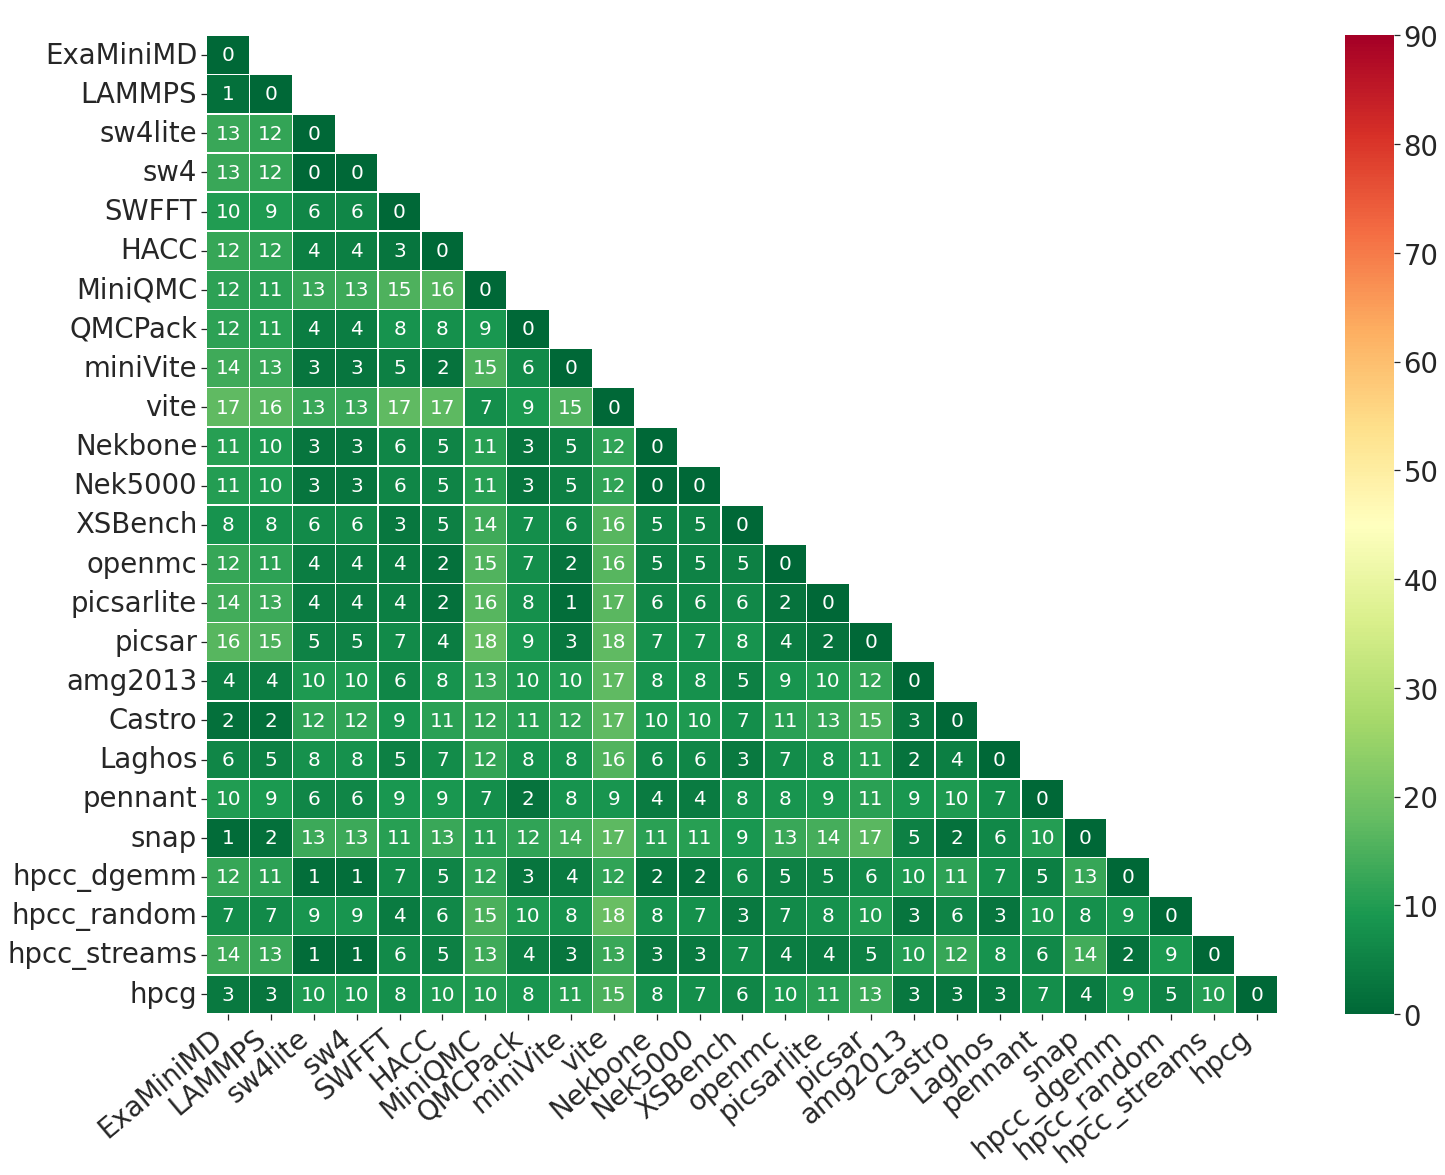
\includegraphics[width=0.9\linewidth]{figs/Branch.png}
\caption{Cosine Similarity for Branch }
\label{figs:cosine Branch}
\end{figure} 

\begin{figure}[ht]
\centering
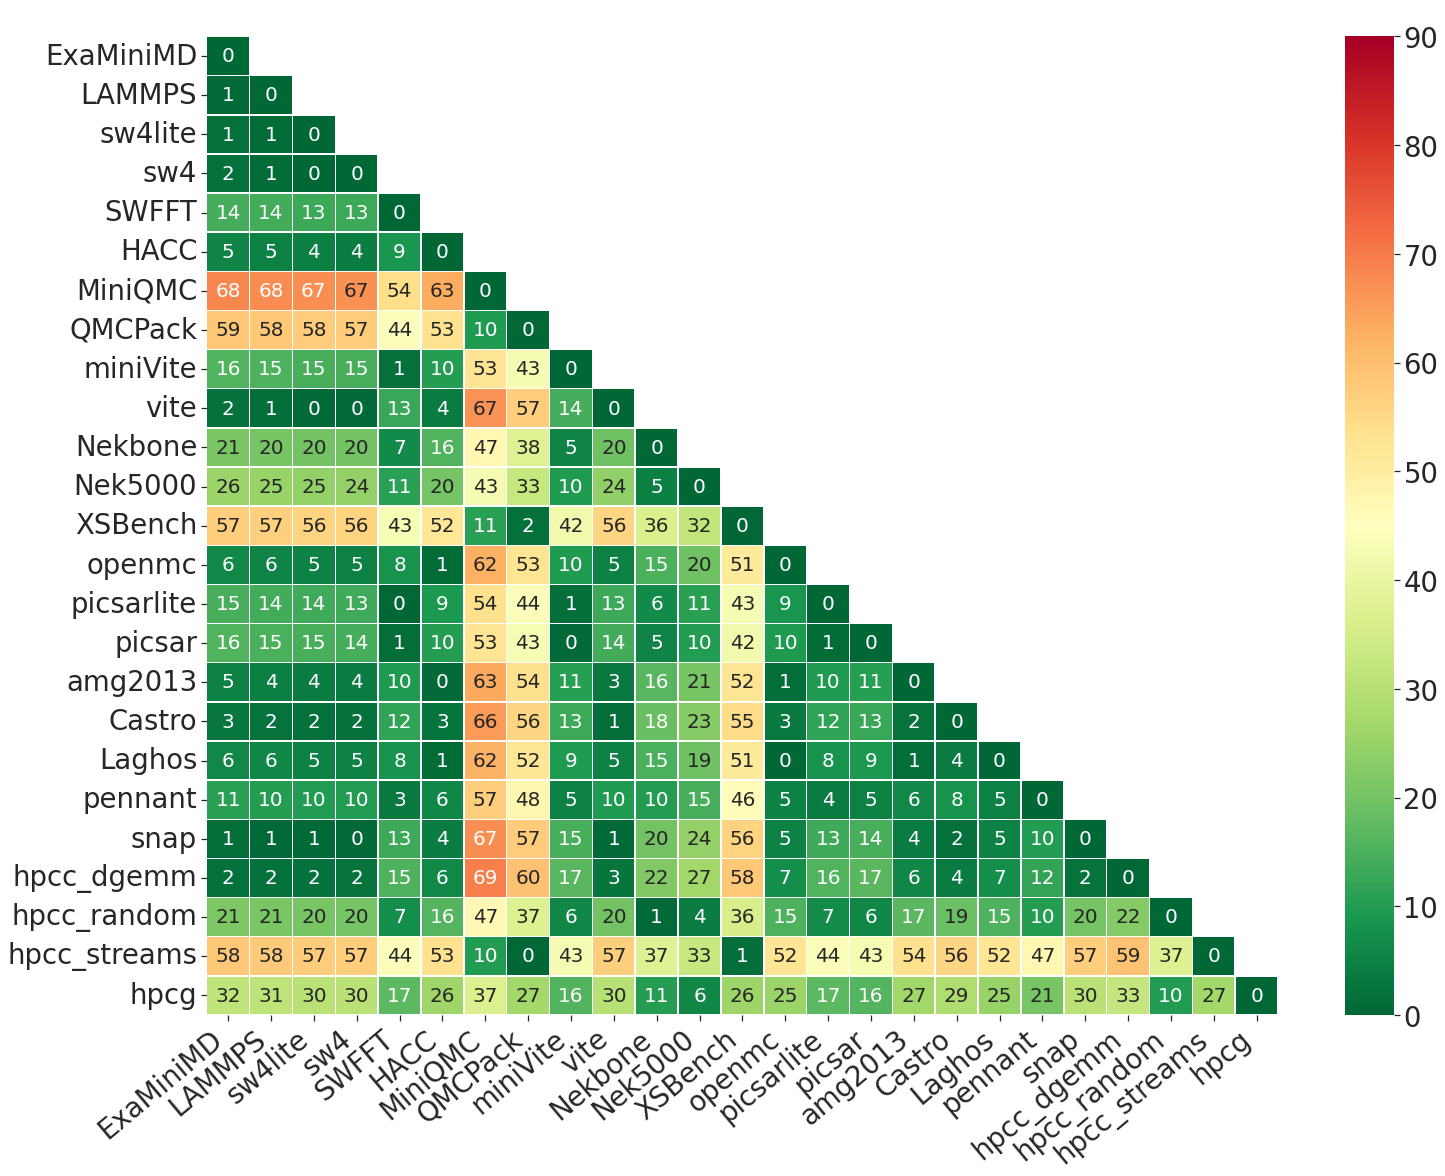
\includegraphics[width=0.9\linewidth]{figs/DecodeIssue_Pipeline.png}
\caption{Cosine Similarity for DecodeIssue Pipeline }
\label{figs:cosine DecodeIssue_Pipeline}
\end{figure}

\begin{figure}[ht]
\centering
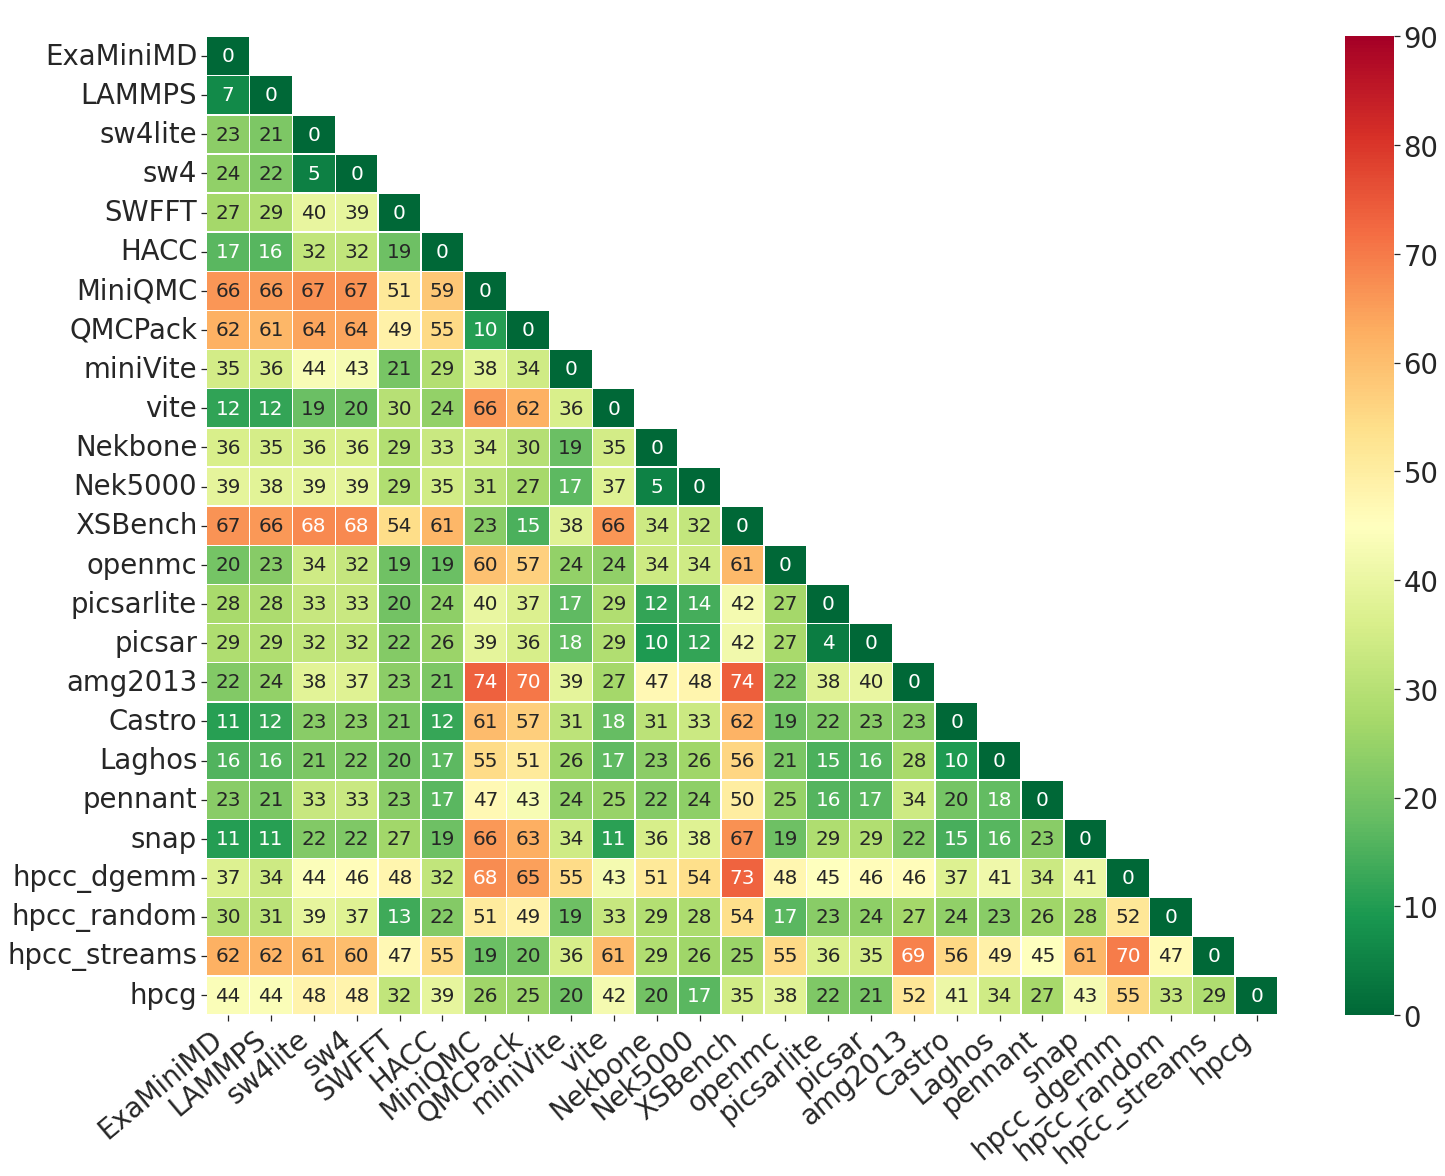
\includegraphics[width=0.9\linewidth]{figs/Dispatch_Pipeline.png}
\caption{Cosine Similarity for Dispatch Pipeline }
\label{figs:cosine Dispatch_Pipeline}
\end{figure}



\begin{figure}[ht]
\centering
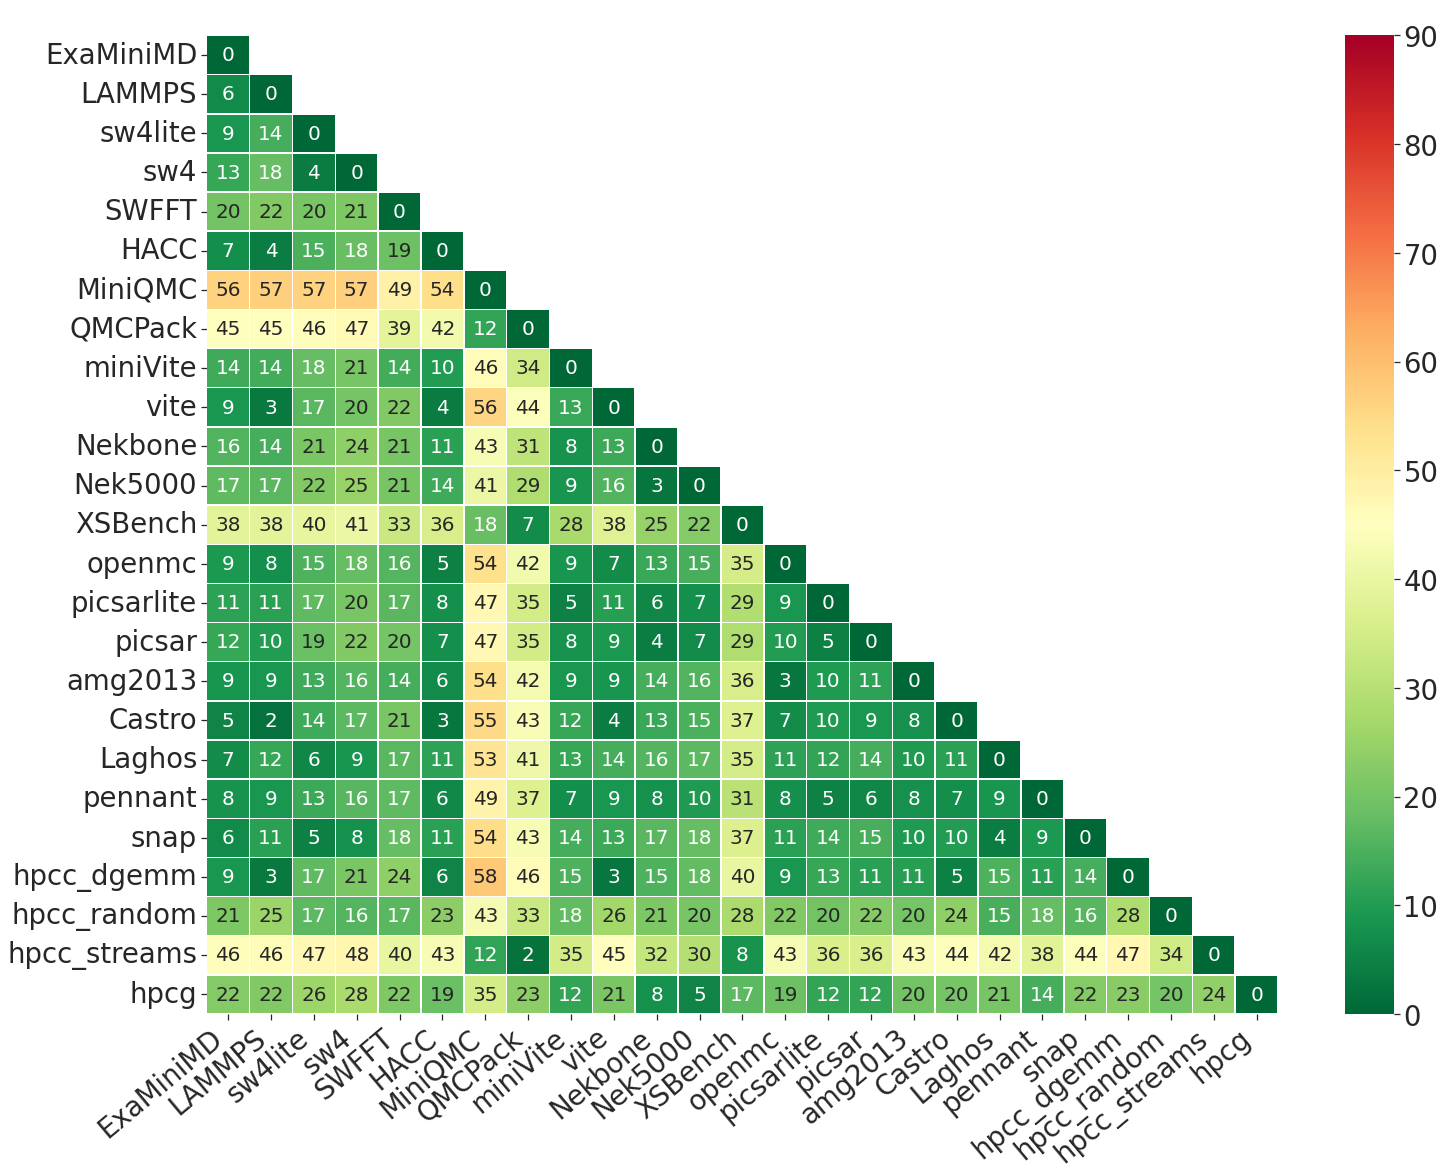
\includegraphics[width=0.9\linewidth]{figs/Frontend.png}
\caption{Cosine Similarity for Frontend }
\label{figs:cosine Frontend}
\end{figure}

\begin{figure}[ht]
\centering
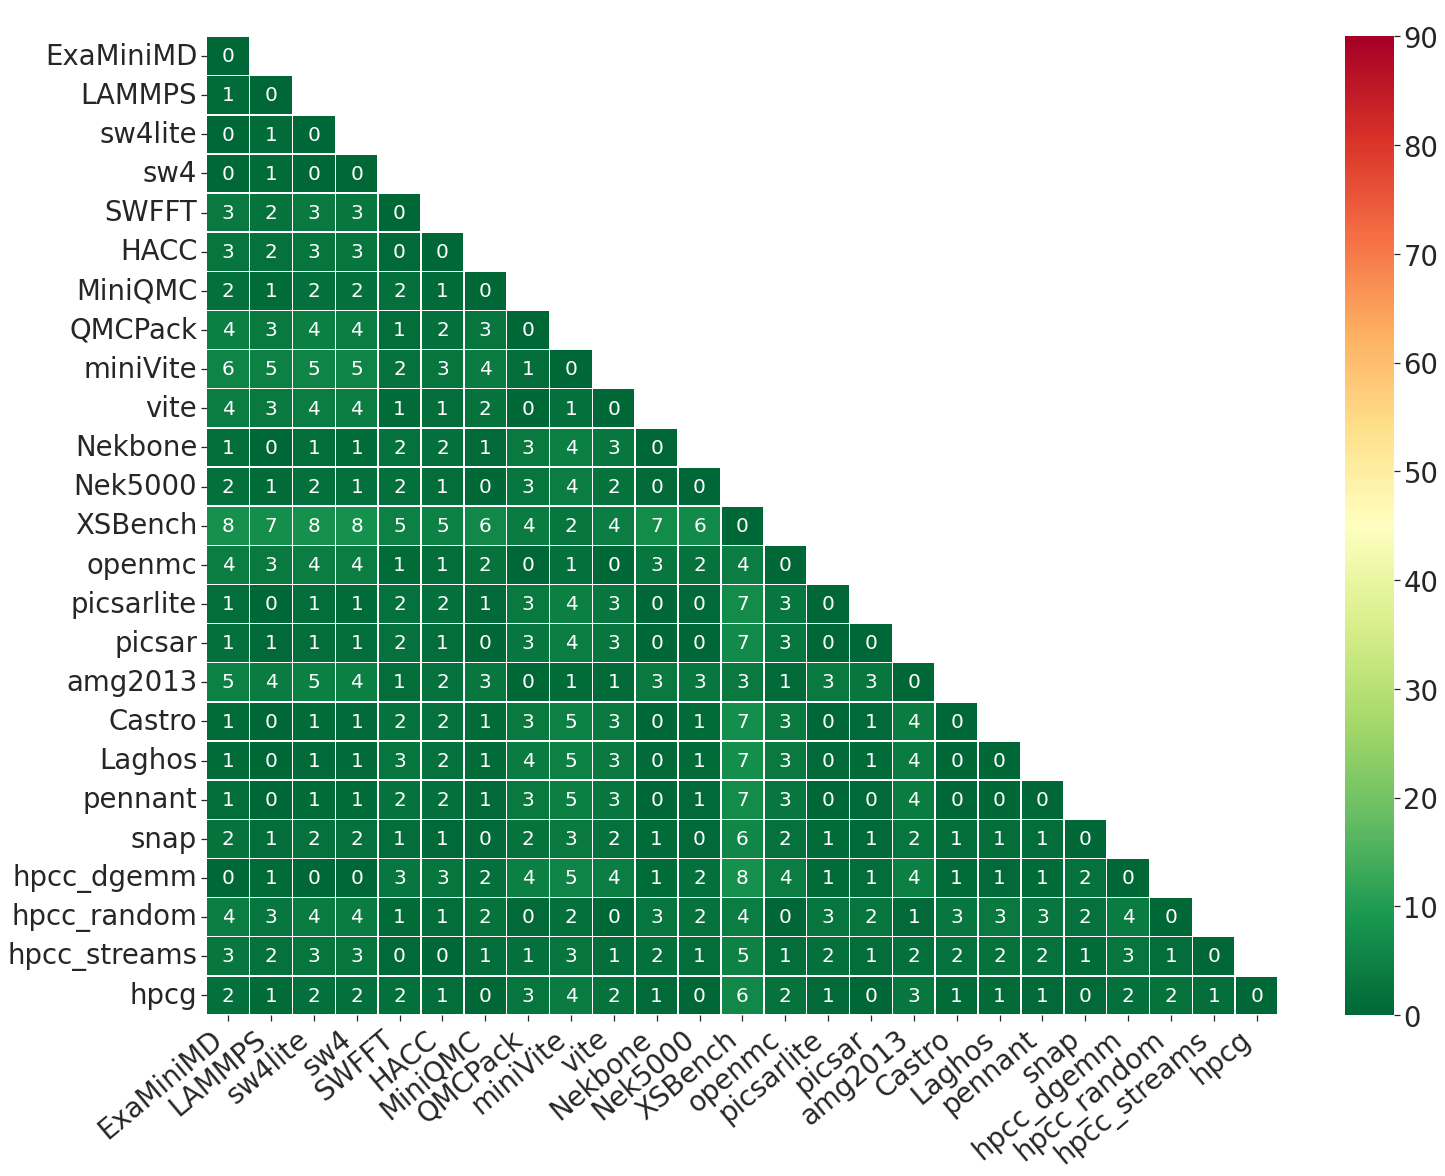
\includegraphics[width=0.9\linewidth]{figs/Instruction_Cache.png}
\caption{Cosine Similarity for Instruction Cache }
\label{figs:cosine Instruction_Cache}
\end{figure}

\begin{figure}[ht]
\centering
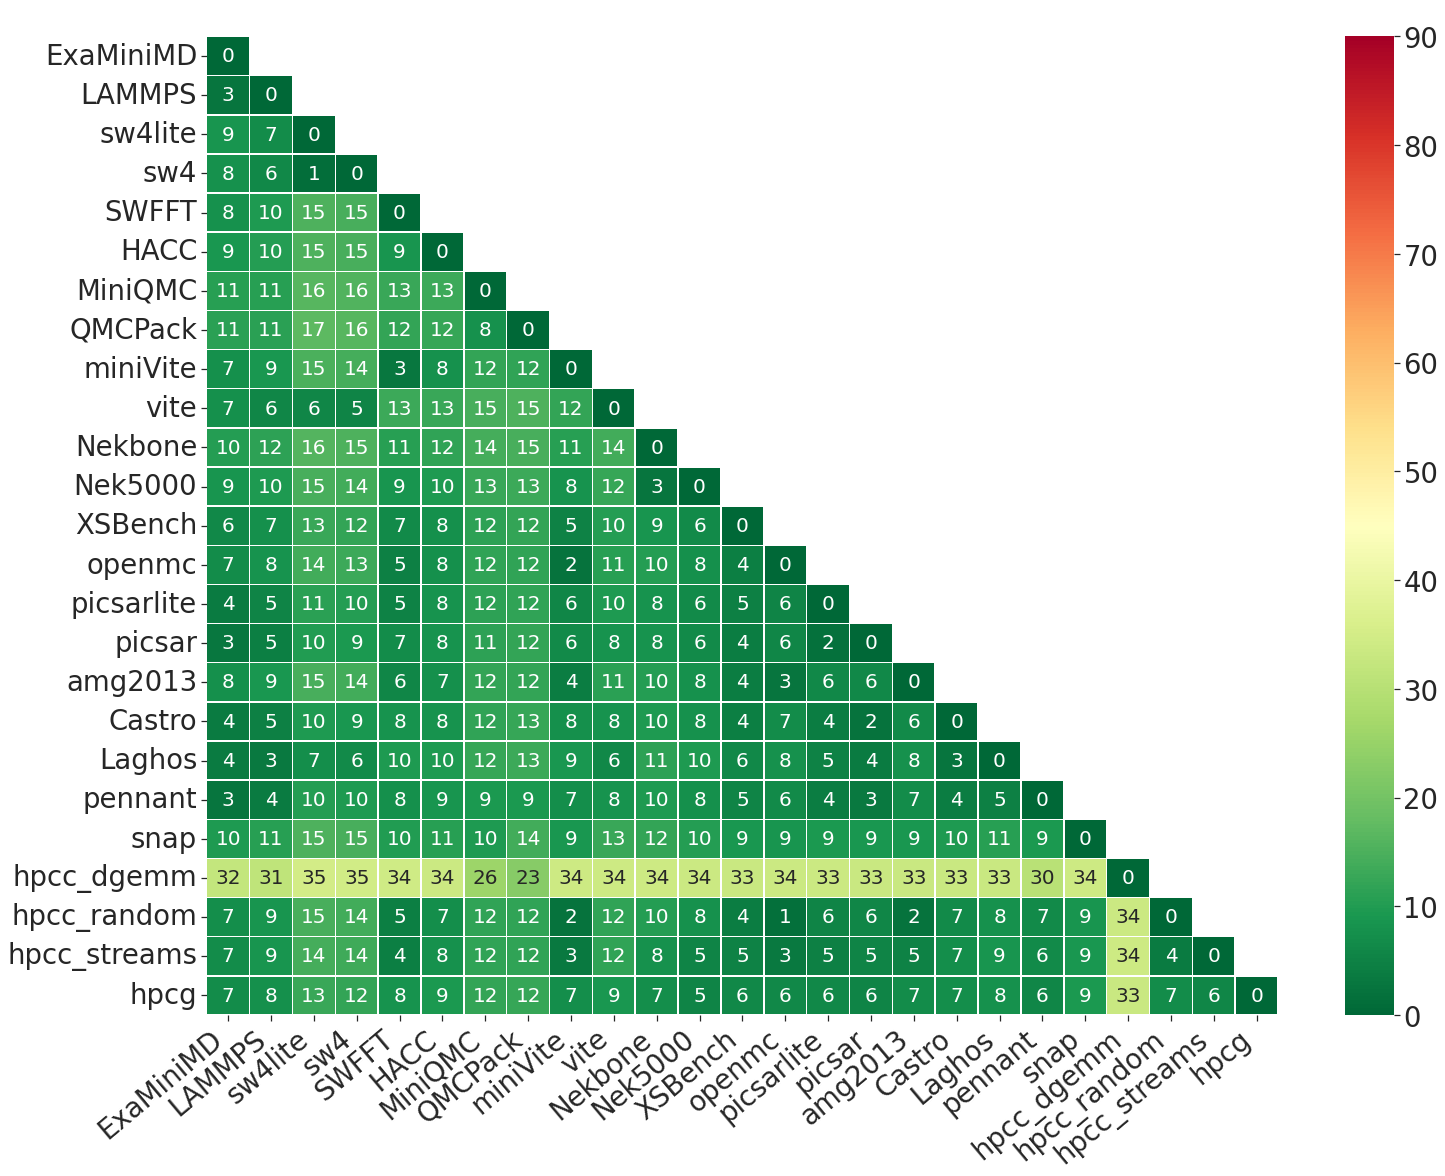
\includegraphics[width=0.9\linewidth]{figs/Instruction_Mix.png}
\caption{Cosine Similarity for Instruction Mix }
\label{figs:cosine Instruction_Mix}
\end{figure}

\begin{figure}[ht]
\centering
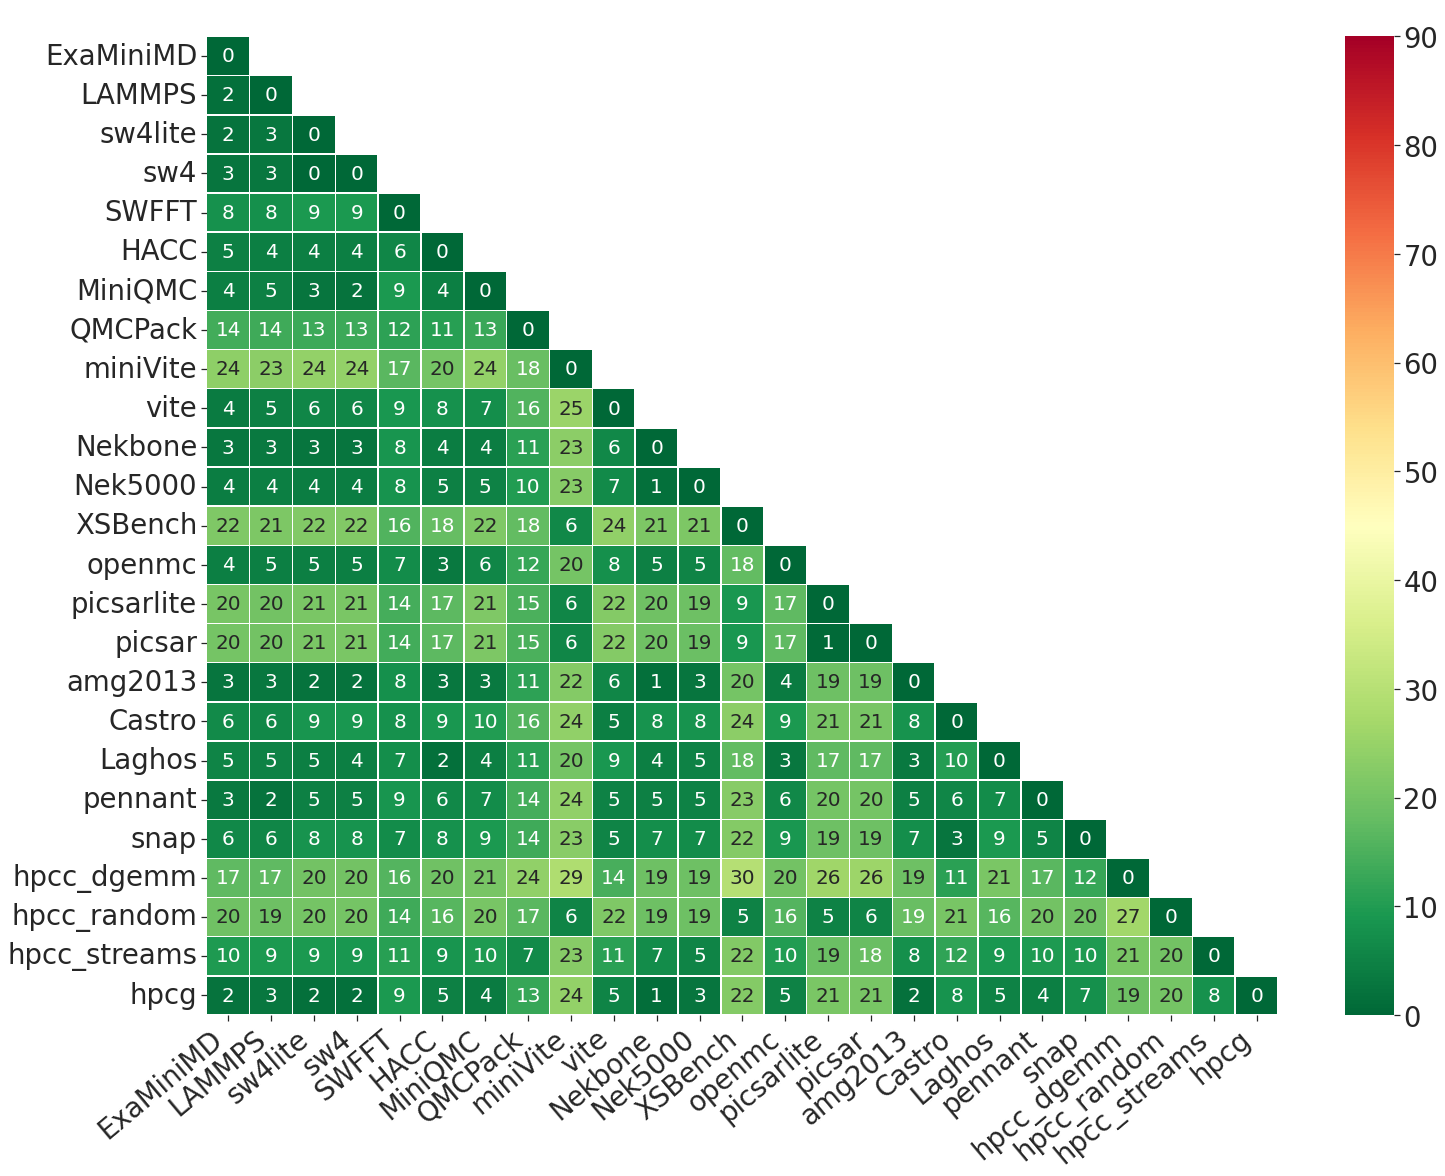
\includegraphics[width=0.9\linewidth]{figs/L3_D_Cache.png}
\caption{Cosine Similarity for L3 Cache }
\label{figs:L3_D_Cache}
\end{figure}

\begin{figure}[ht]
\centering
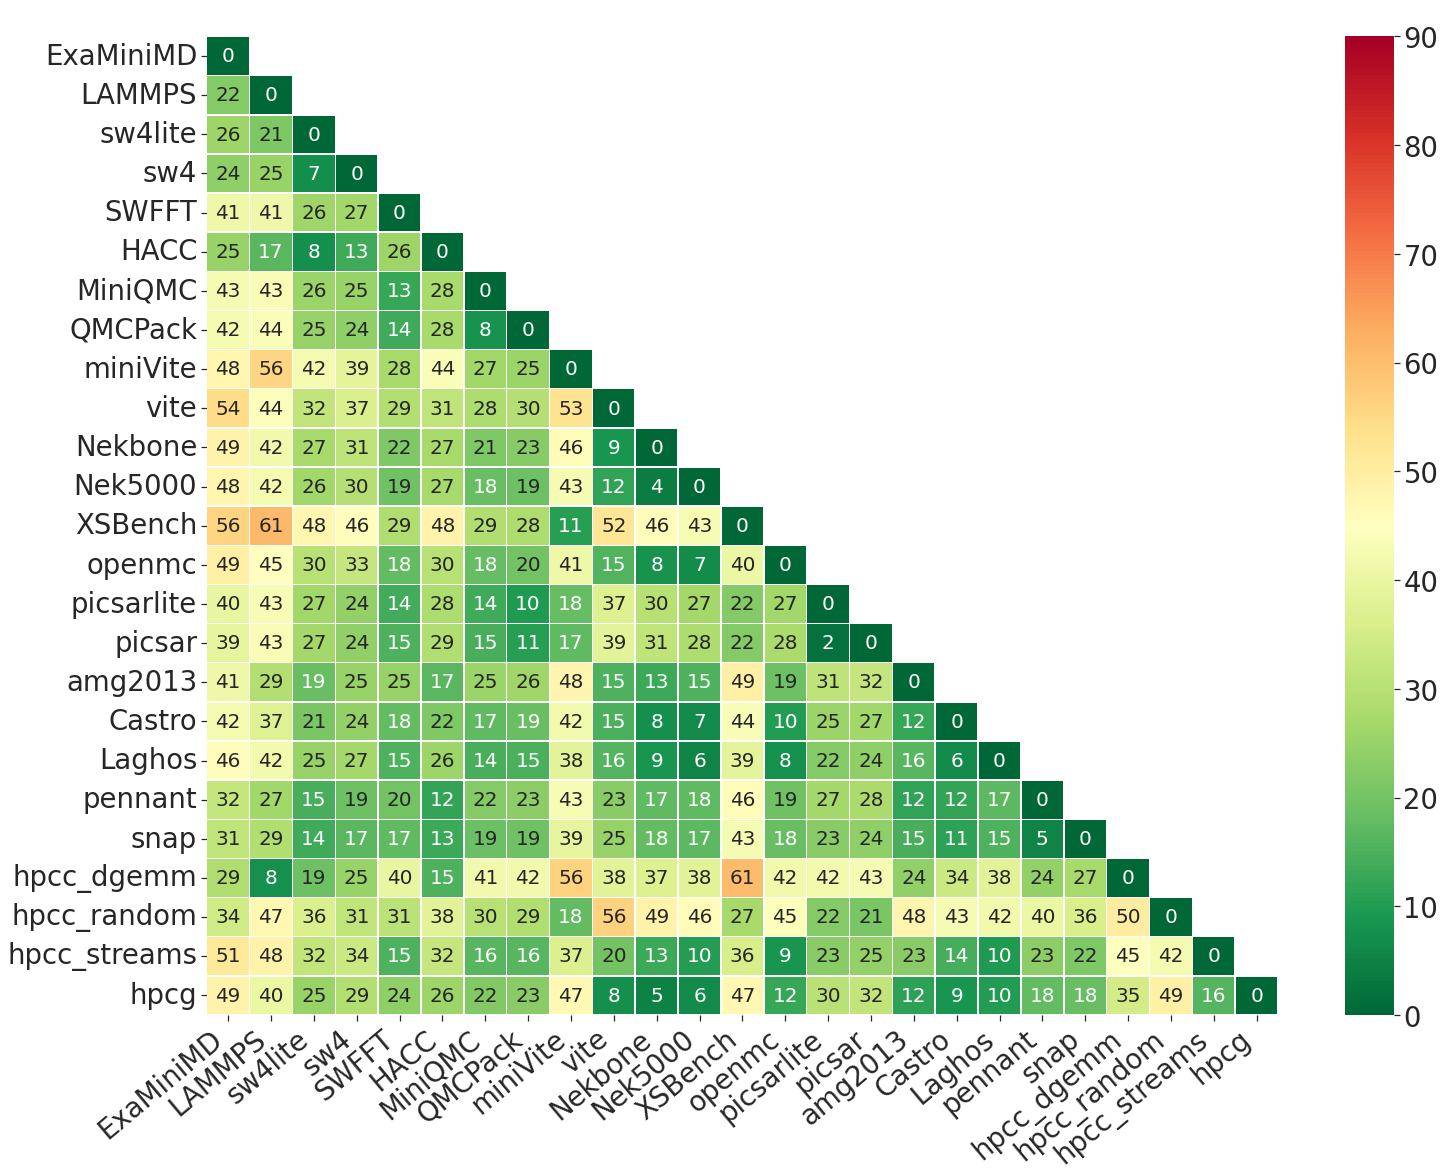
\includegraphics[width=0.9\linewidth]{figs/L2_D_Cache.png}
\caption{Cosine Similarity for L2 Cache }
\label{figs:cosine L2_D_Cache}
\end{figure}



\begin{figure}[ht]
\centering
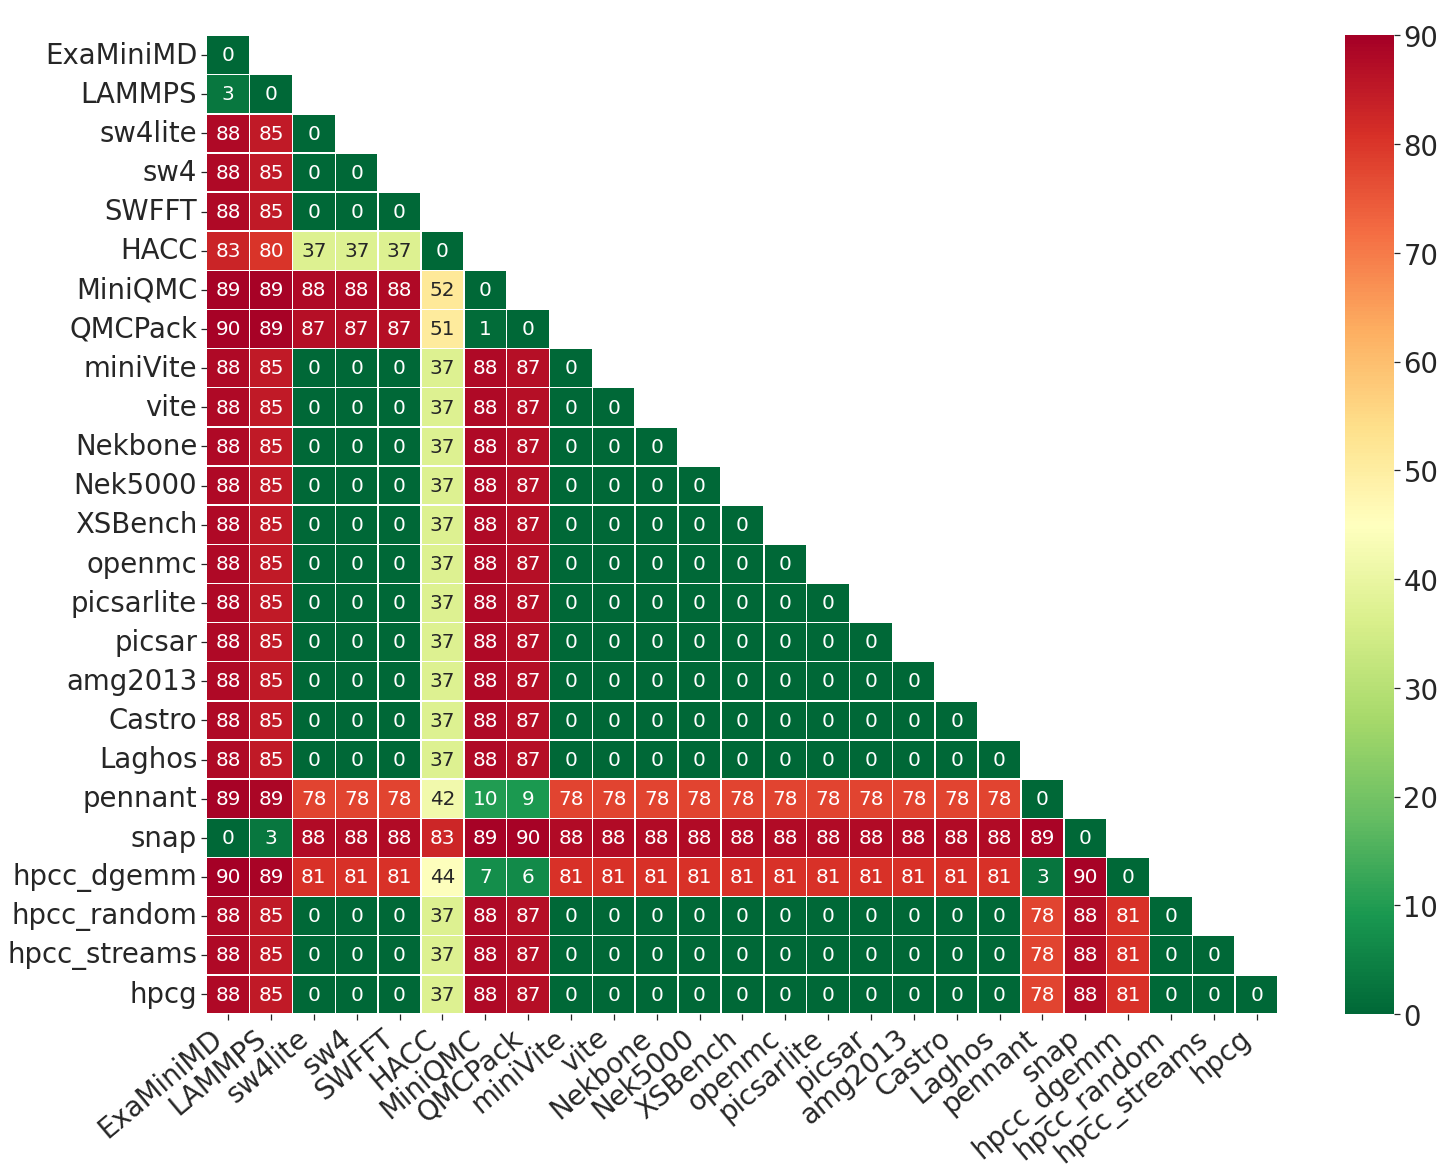
\includegraphics[width=0.9\linewidth]{figs/Power.png}
\caption{Cosine Similarity for Power }
\label{figs:cosine Power}
\end{figure}

\begin{figure}[ht]
\centering
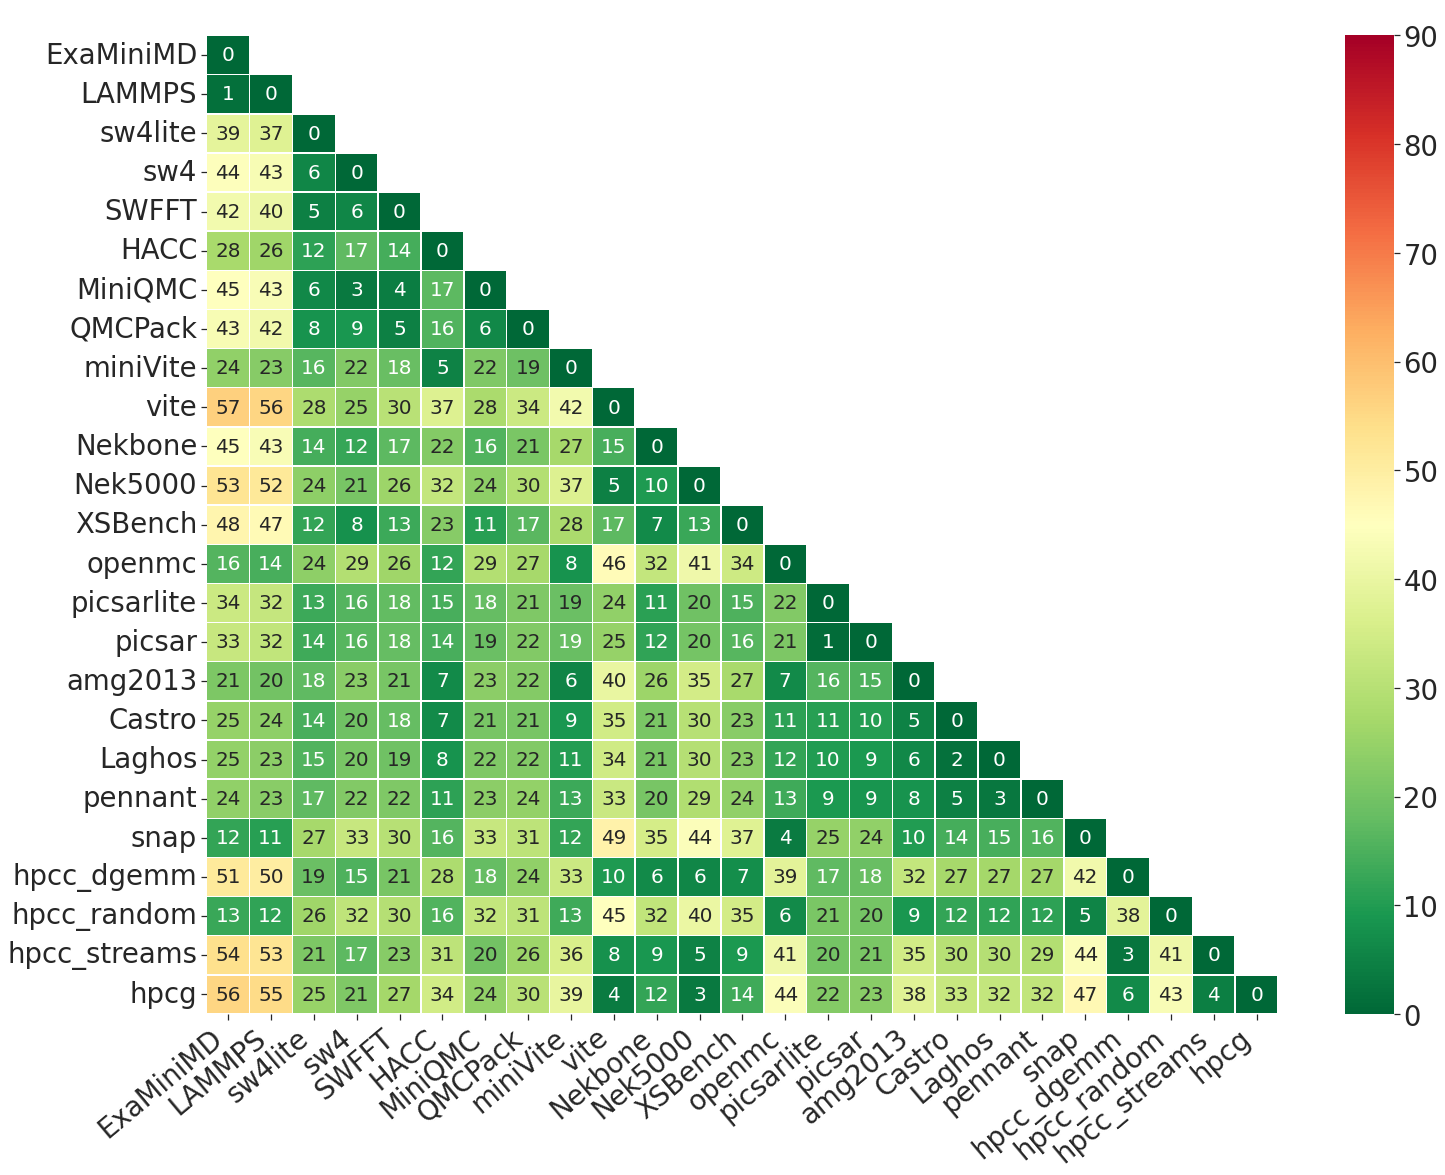
\includegraphics[width=0.9\linewidth]{figs/Misc.png}
\caption{Cosine Similarity for Misc }
\label{figs:cosine Misc}
\end{figure}



\begin{figure}[ht]
\centering
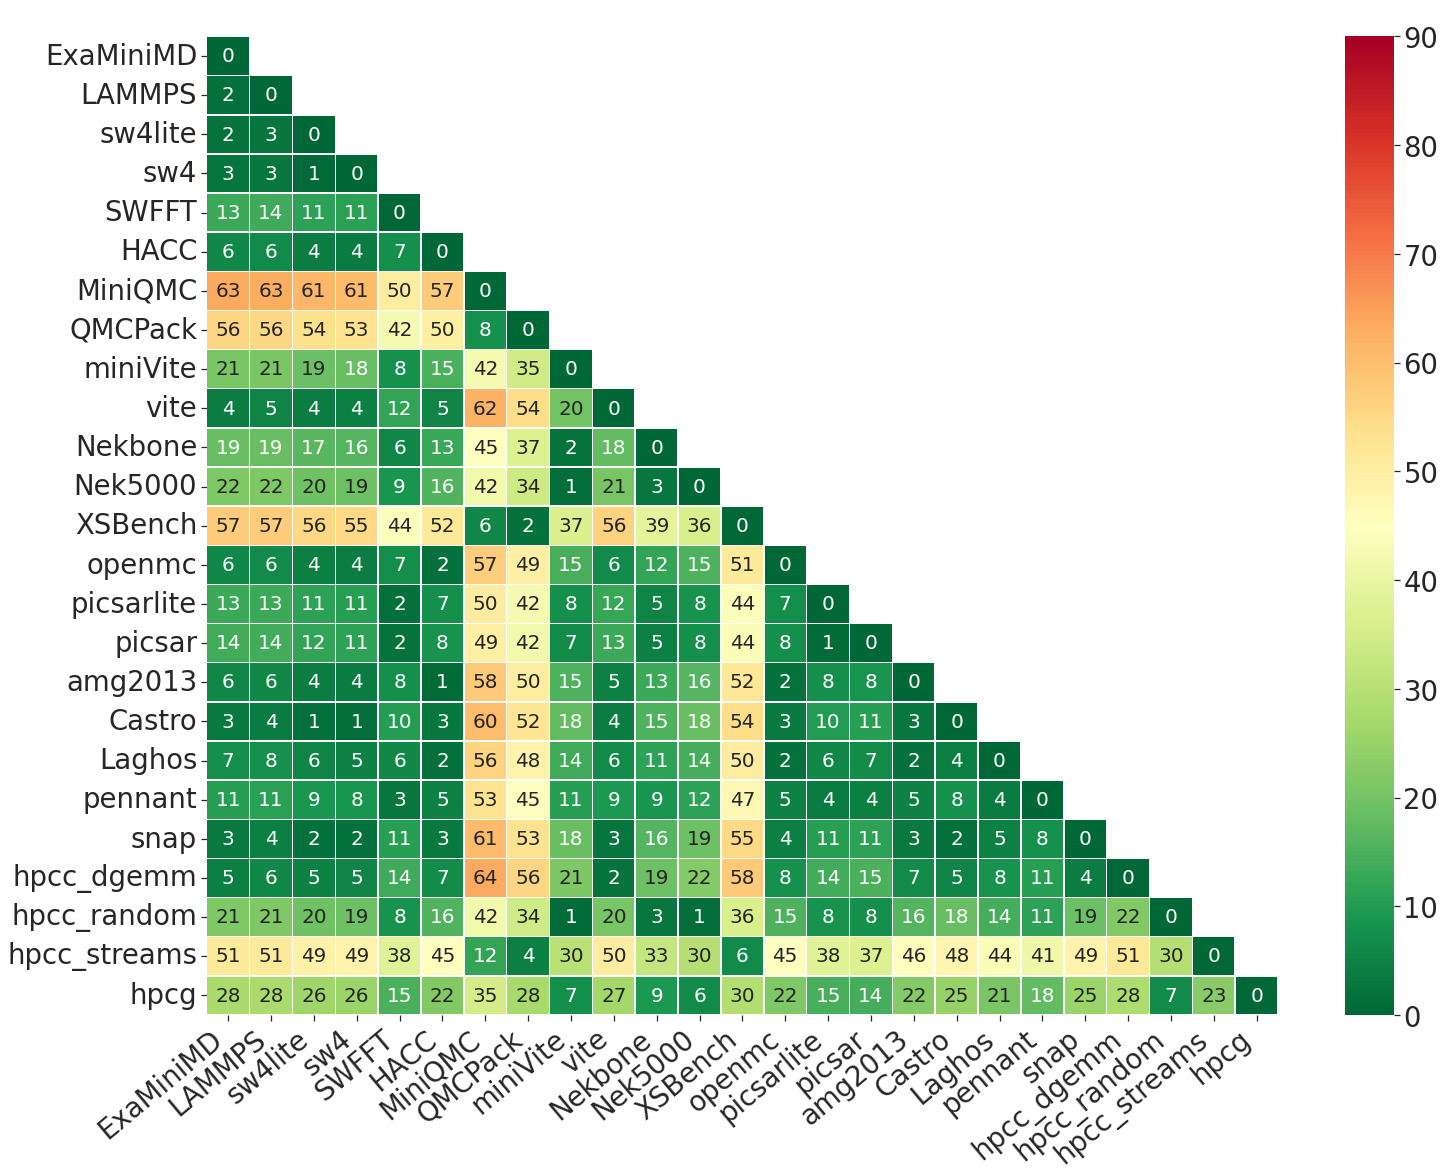
\includegraphics[width=0.9\linewidth]{figs/Retirement_Pipeline.png}
\caption{Cosine Similarity for Retirement Pipeline }
\label{figs:cosine Retirement_Pipeline}
\end{figure}

\begin{figure}[ht]
\centering
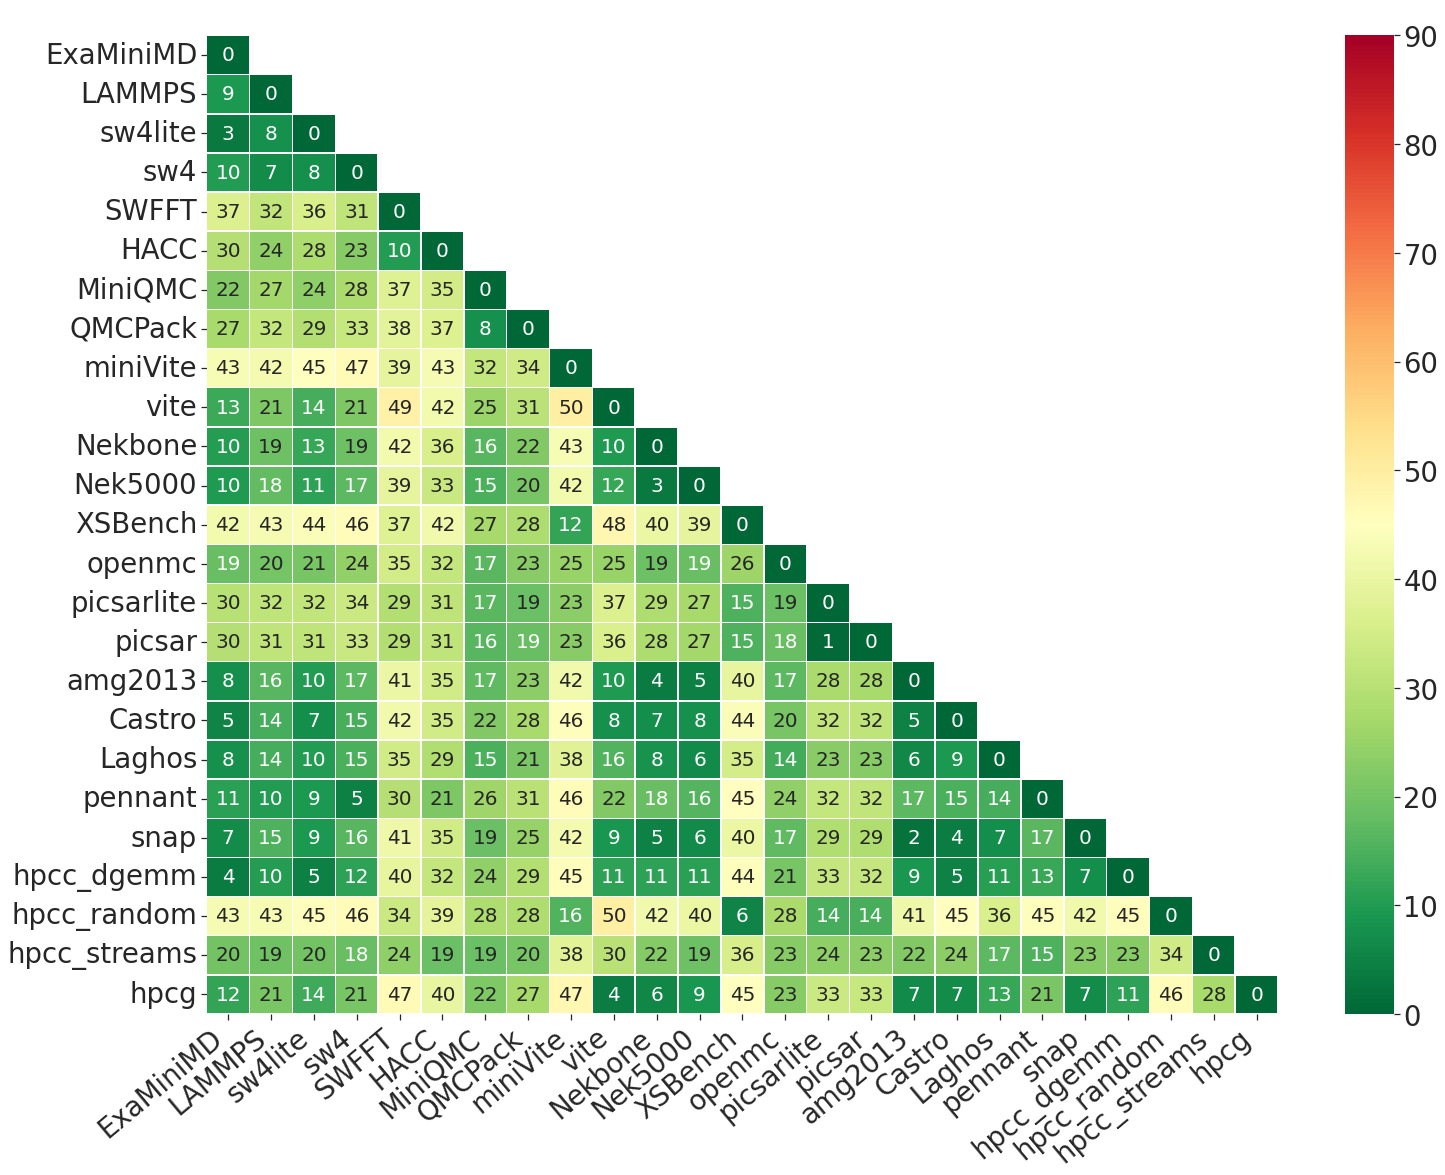
\includegraphics[width=0.9\linewidth]{figs/Memory.png}
\caption{Cosine Similarity for Memory }
\label{figs:cosine Memory}
\end{figure}

\end{appendices}

\end{document}